\section{An axisymmetric potential for a cosmological simulation.}
Code from Timo Halbesma, Federico Marinacci, Rob Grand, Wilma Trick


\subsection{About Auriga}
\subsubsection{Hydrodynamical galaxy simulations}
To understand how our Universe and everything in it has formed and evolved, astronomers use simulations of it two ways: trying to match observations of real galaxies and thus checking if the input 'recipes' are correct and predicting observations which then are to be found by observers. These simulations stretch over a large range of astronomical scales, from stars and planets to the evolution of the cosmic web, but also over different numerical techniques, from more empirical, statistical Monte-Carlo methods to cosmological hydrodynamical \textit{N}-body simulations. To learn more about the formation and evolution of galaxies, these hydrodynamical cosmological simulations are a wealthy tool to exploit. 


\\This work focuses on the Auriga \citep{AurigaGrand} simulations, which try to recreate spiral galaxies such as our own. 

\subsubsection{Auriga}
Auriga \citep{AurigaGrand} is a magnetohydrodynamical zoom-in simulation of an isolated \ac{MW} like galaxy. It is build with AREPO \citep{AREPO} and includes galaxy physics, \ac{AGN} feedback and magnetic fields. Its goal is to match the observables of the \ac{MW} today and to produce its history which can be compared to observations of spiral galaxies in earlier stages of development. The snapshots go from redshift 127, which is close to the beginning of the universe, to redshift 0, today. All 30 galaxies are run in normal resolution and 3 selected are run in low and high resolution as well. At redshift = 0, different galaxy shapes are evolved. Most of them are spirals but a few are in a merger process. All galaxies have a rich merger history.


\begin{figure}
    \centering
    \begin{subfigure}[b]{0.8\textwidth}
	    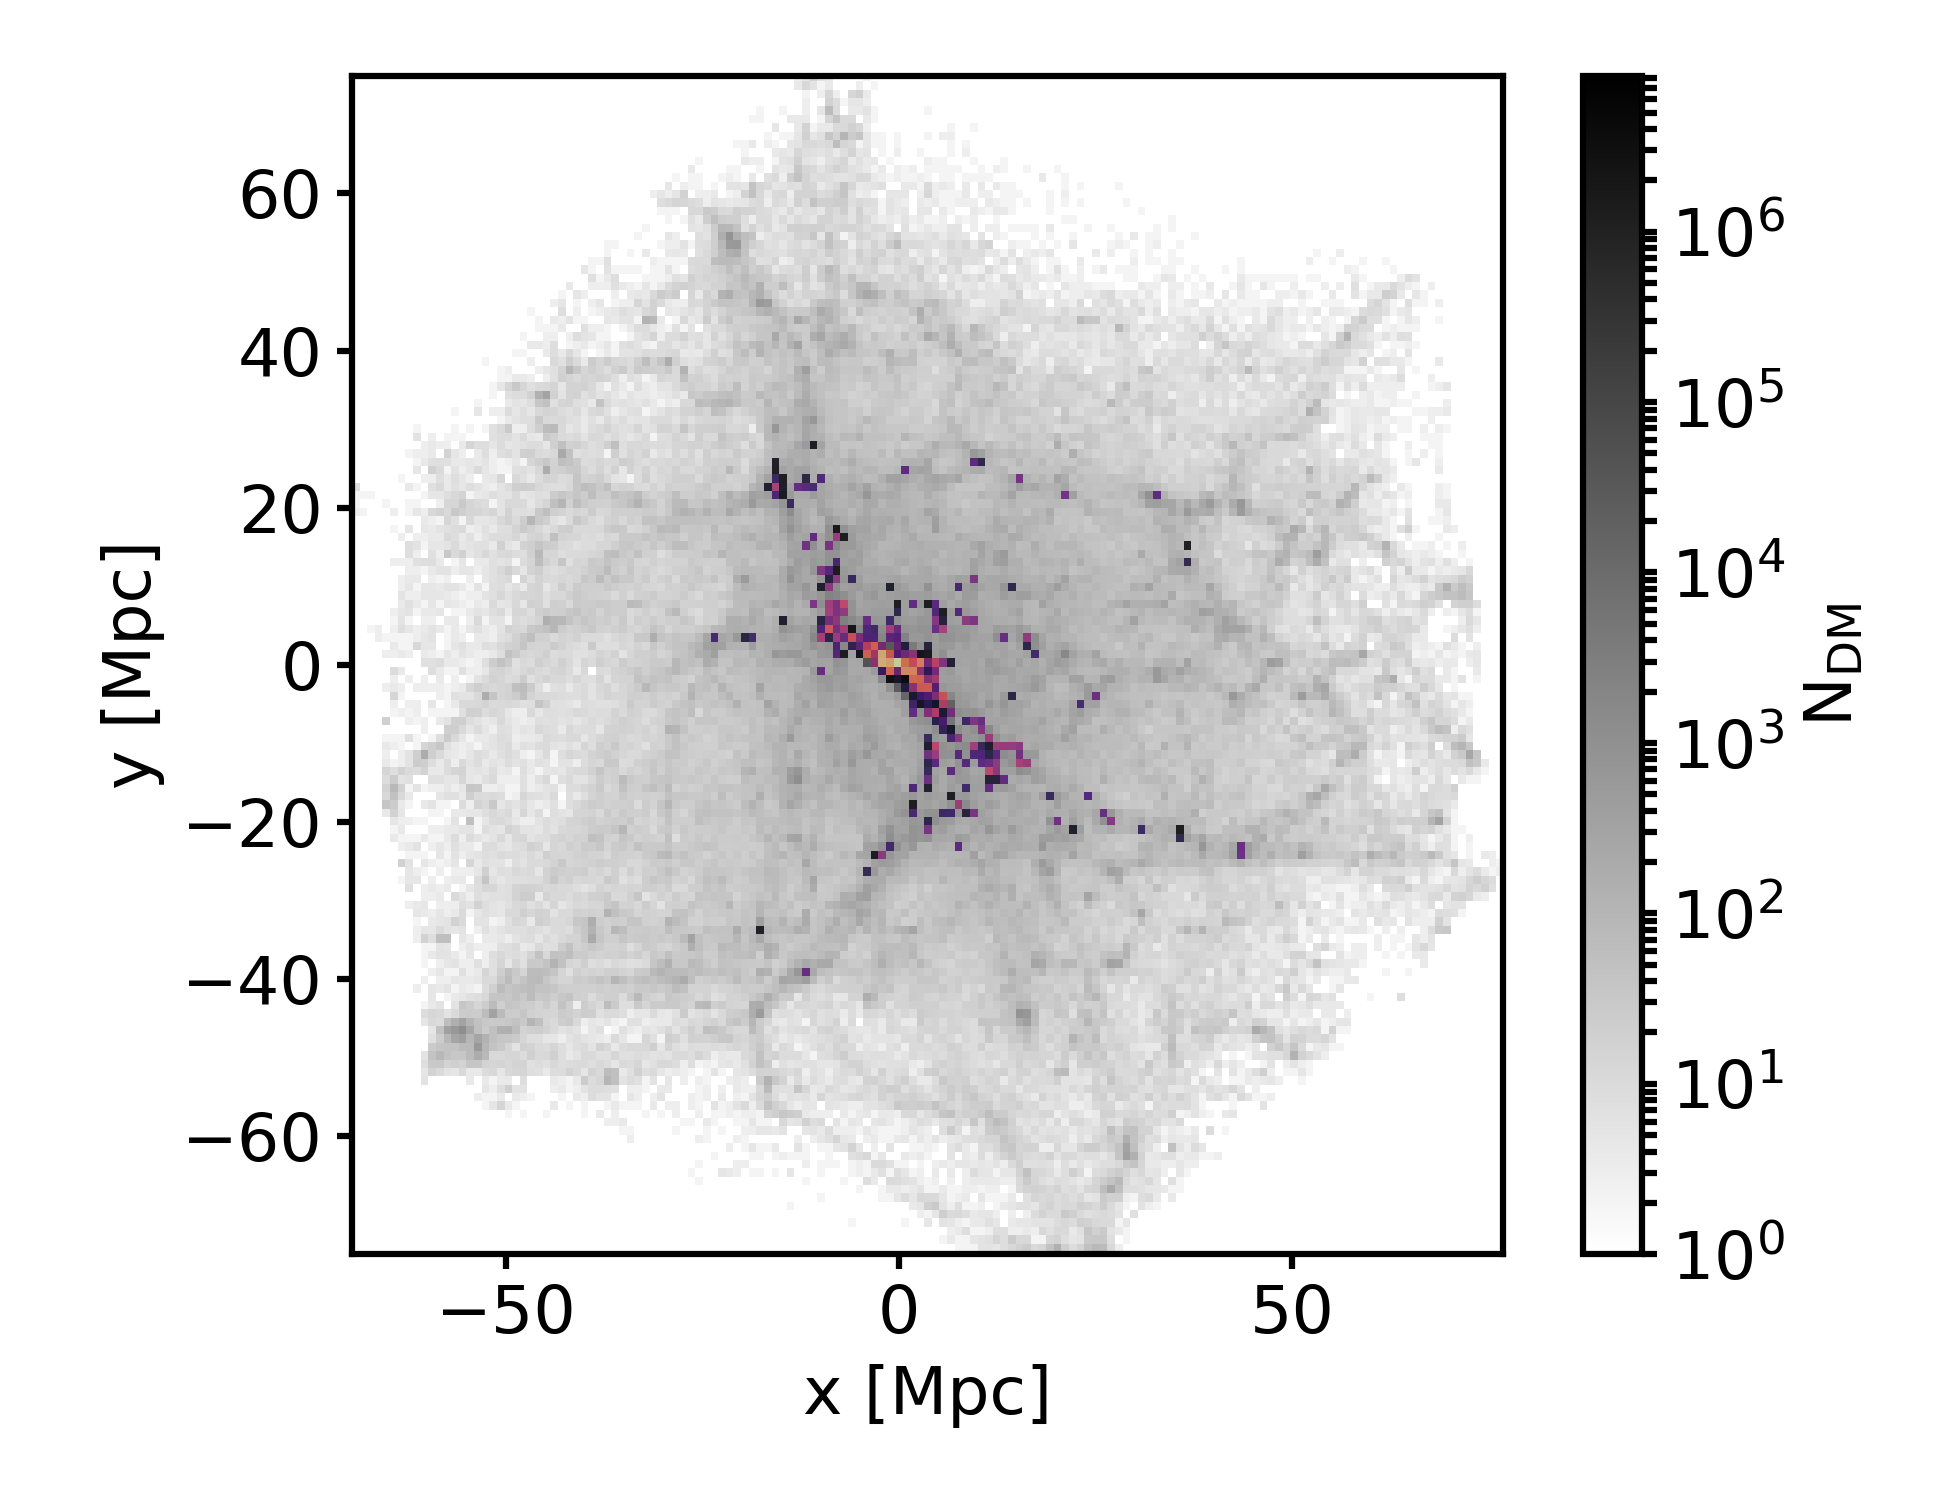
\includegraphics[width=\textwidth]{plots/Auriga/DM_and_stars_xy_distribution.png}
	    \label{fig:DM_stars_xy}
    \end{subfigure}
    
    \begin{subfigure}[b]{0.8\textwidth}
    \centering
    	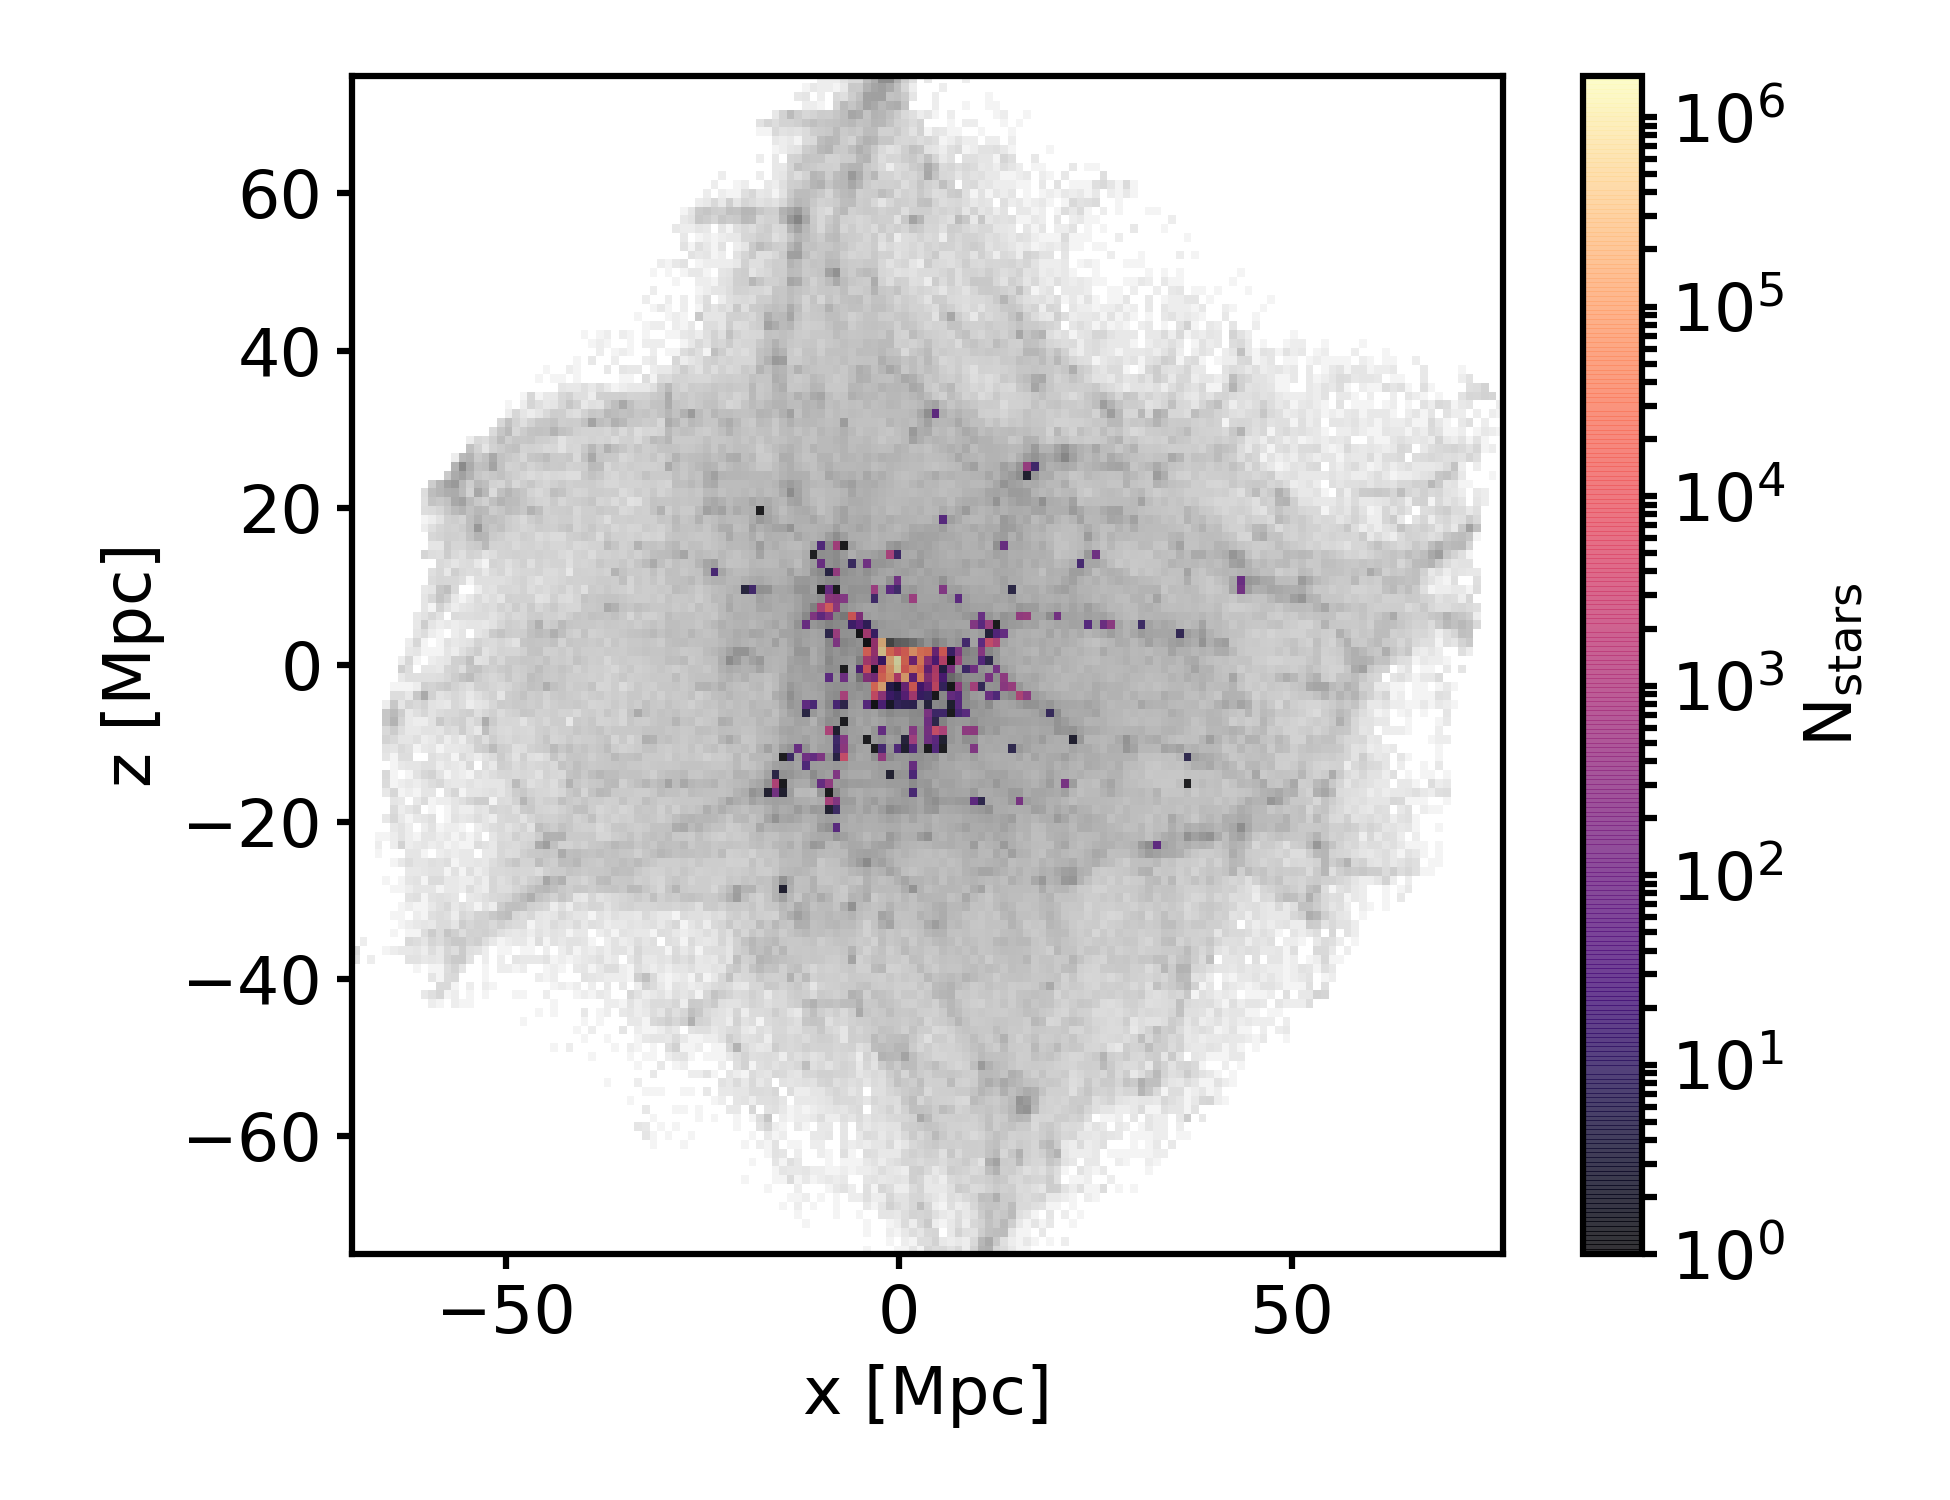
\includegraphics[width=\textwidth]{plots/Auriga/DM_and_stars_xz_distribution.png}
    	\label{fig:DM_stars_xy}
    \end{subfigure}
    \caption{\ac{DM} (grey) and stellar (colors) particle distribution of the whole simulation Auriga24 at $\textit{z}=0$. The \ac{DM} forms the cosmic web, where the mass gathers along its filaments. Baryonic matter also follows these structures. At the most massive parts of the \ac{DM} distribution, the most stellar particles fell in. }\label{fig:DM_stars_AU24}
\end{figure}


\begin{figure}
    \centering
    \begin{subfigure}[b]{0.8\textwidth}
	    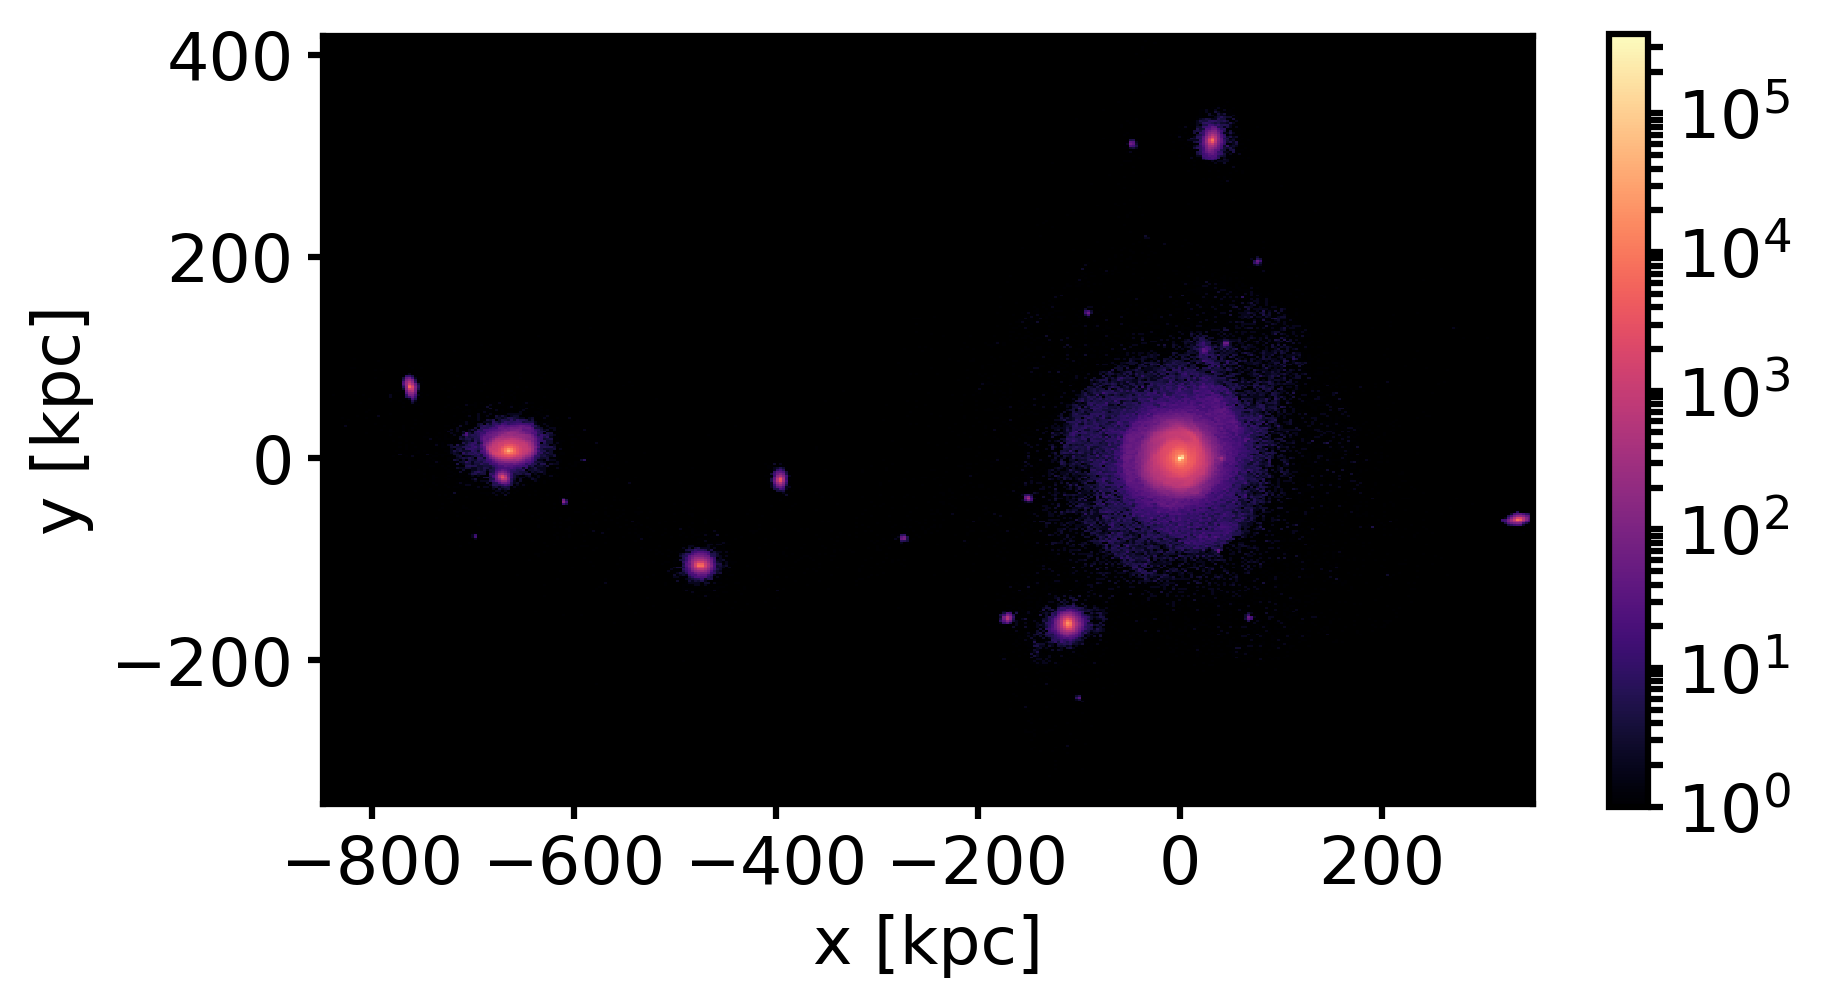
\includegraphics[width=\textwidth]{plots/Auriga/Au24_stars_xy_distribution_halo0.png}
	    \label{fig:Au24_stars_xy}
    \end{subfigure}
    
    \begin{subfigure}[b]{0.8\textwidth}
    \centering
    	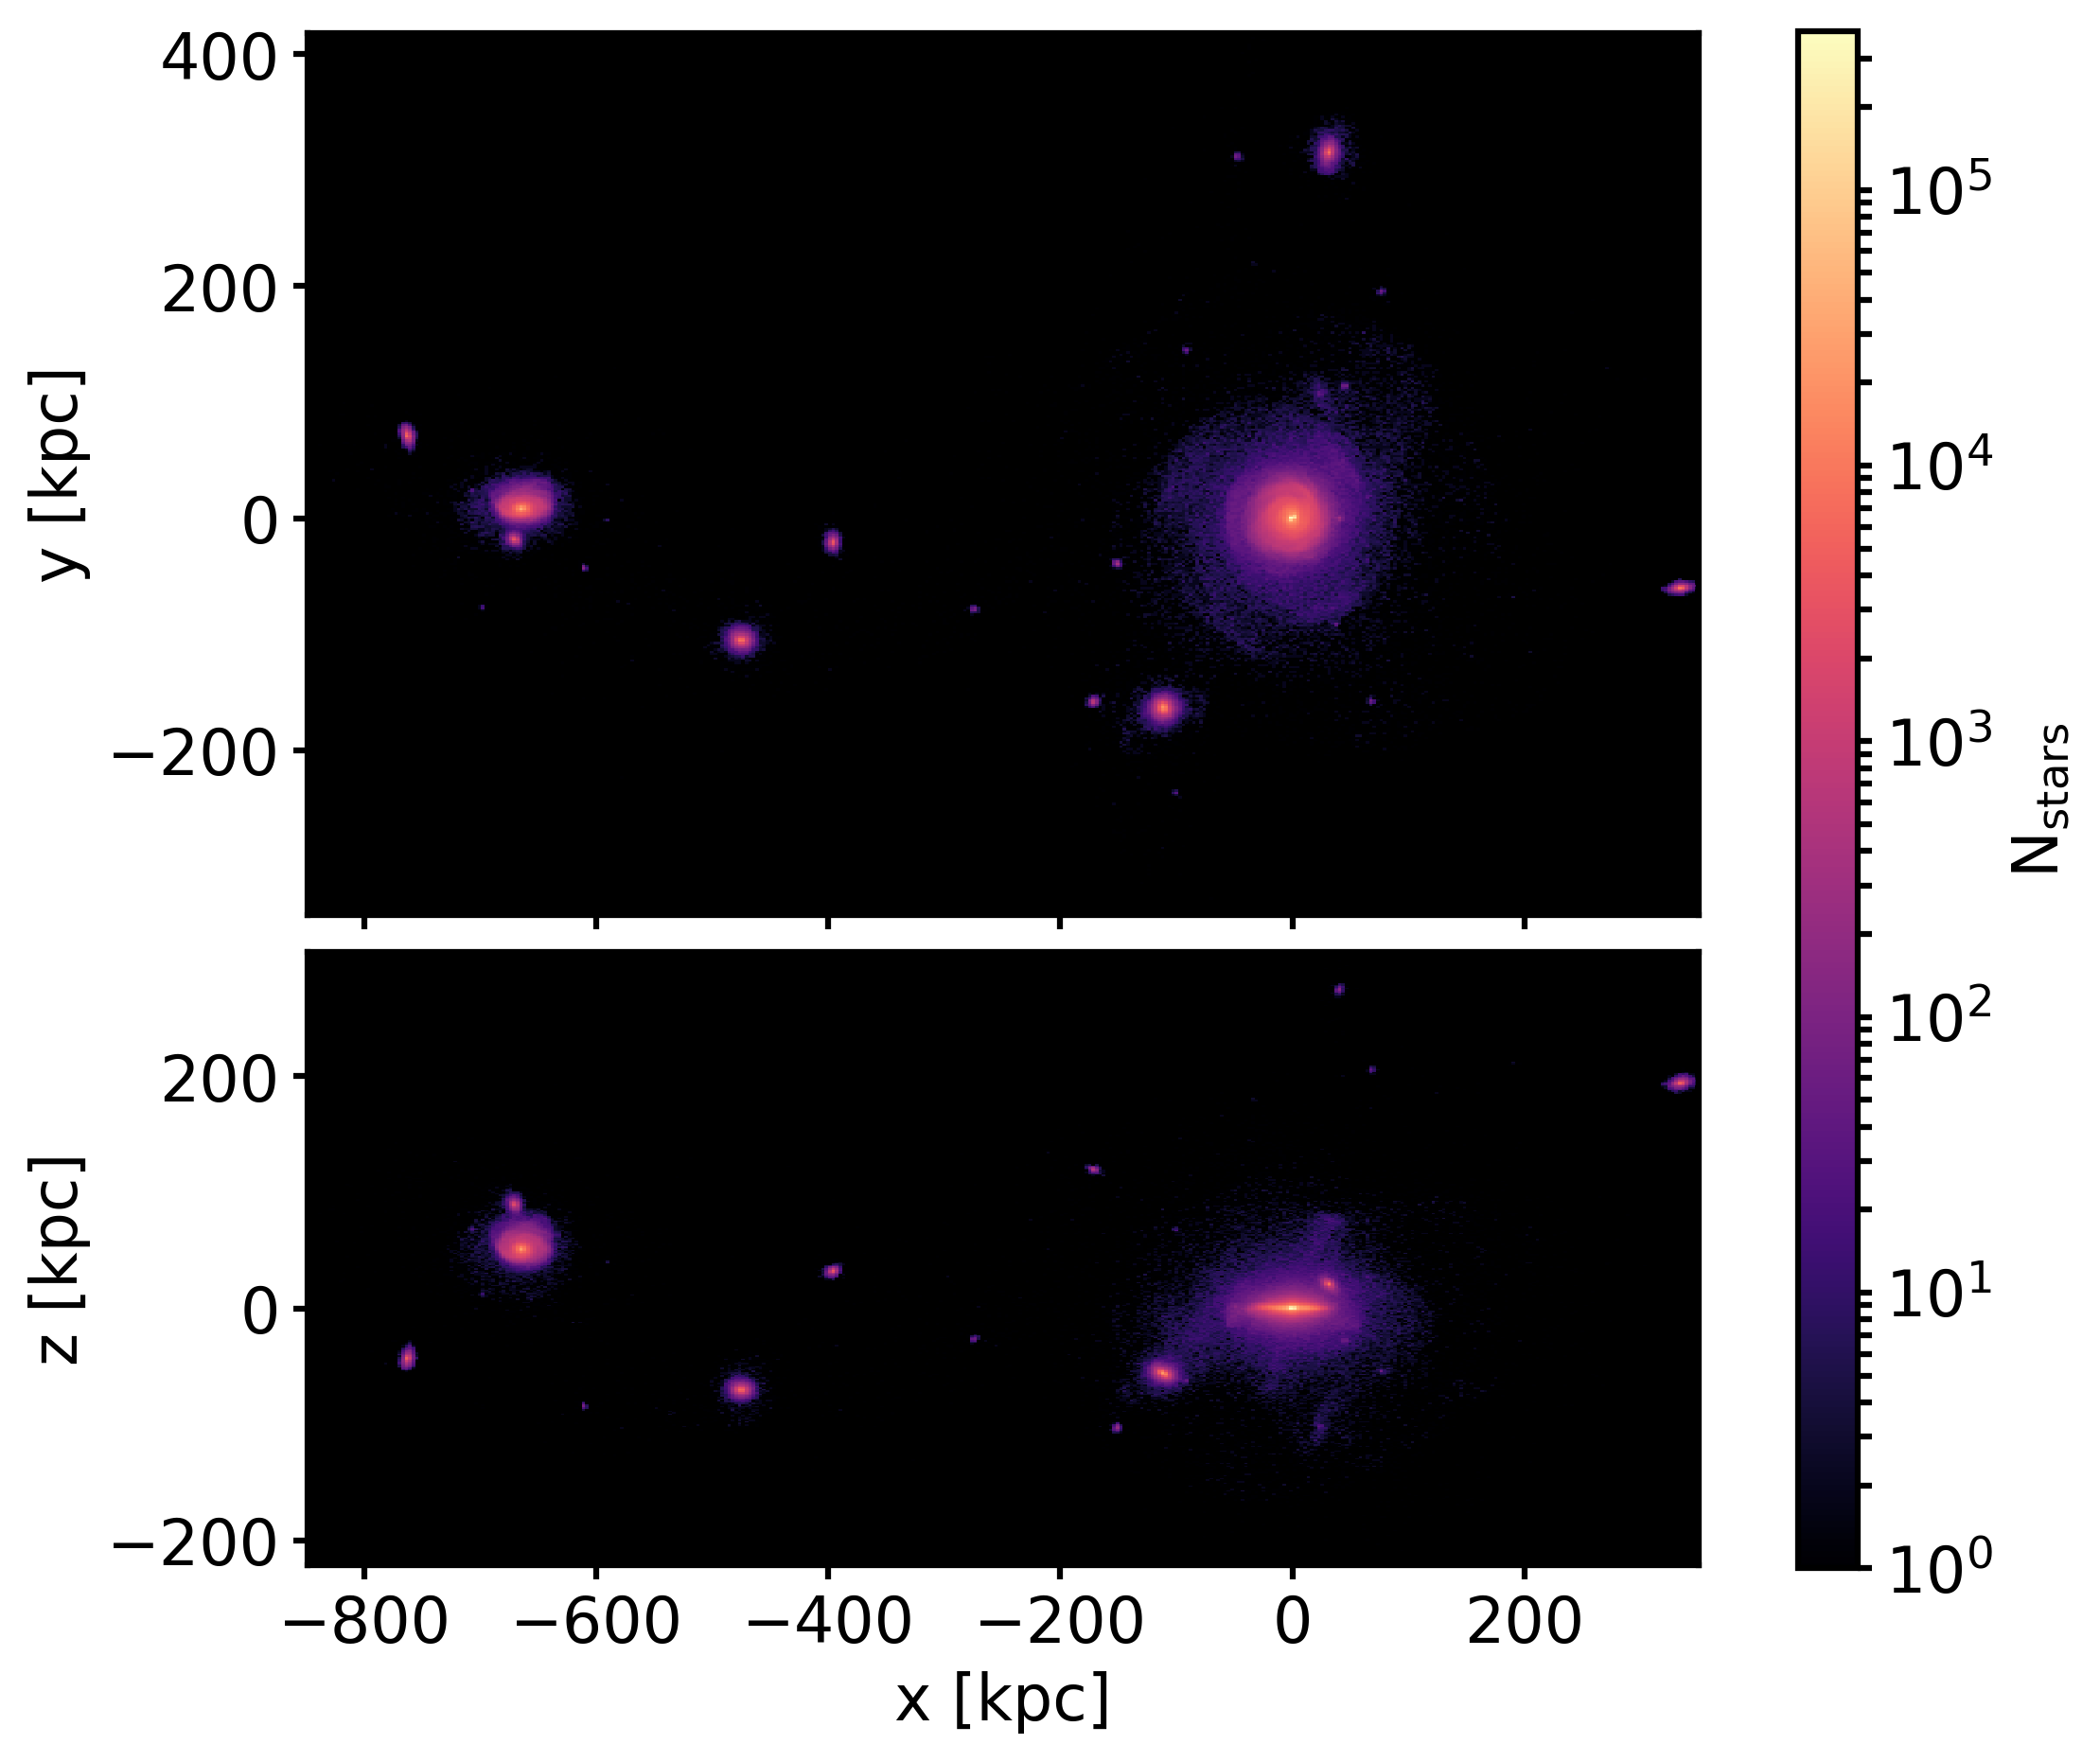
\includegraphics[width=\textwidth]{plots/Auriga/Au24_stars_xz_distribution_halo0.png}
    	\label{fig:Au24_stars_xz}
    \end{subfigure}
    \caption{Stellar distribution of 0th halo at $\textit{z}=0$.}\label{fig:Stars_AU24}
\end{figure}

\begin{figure}
    \centering
    \begin{subfigure}[b]{0.8\textwidth}
	    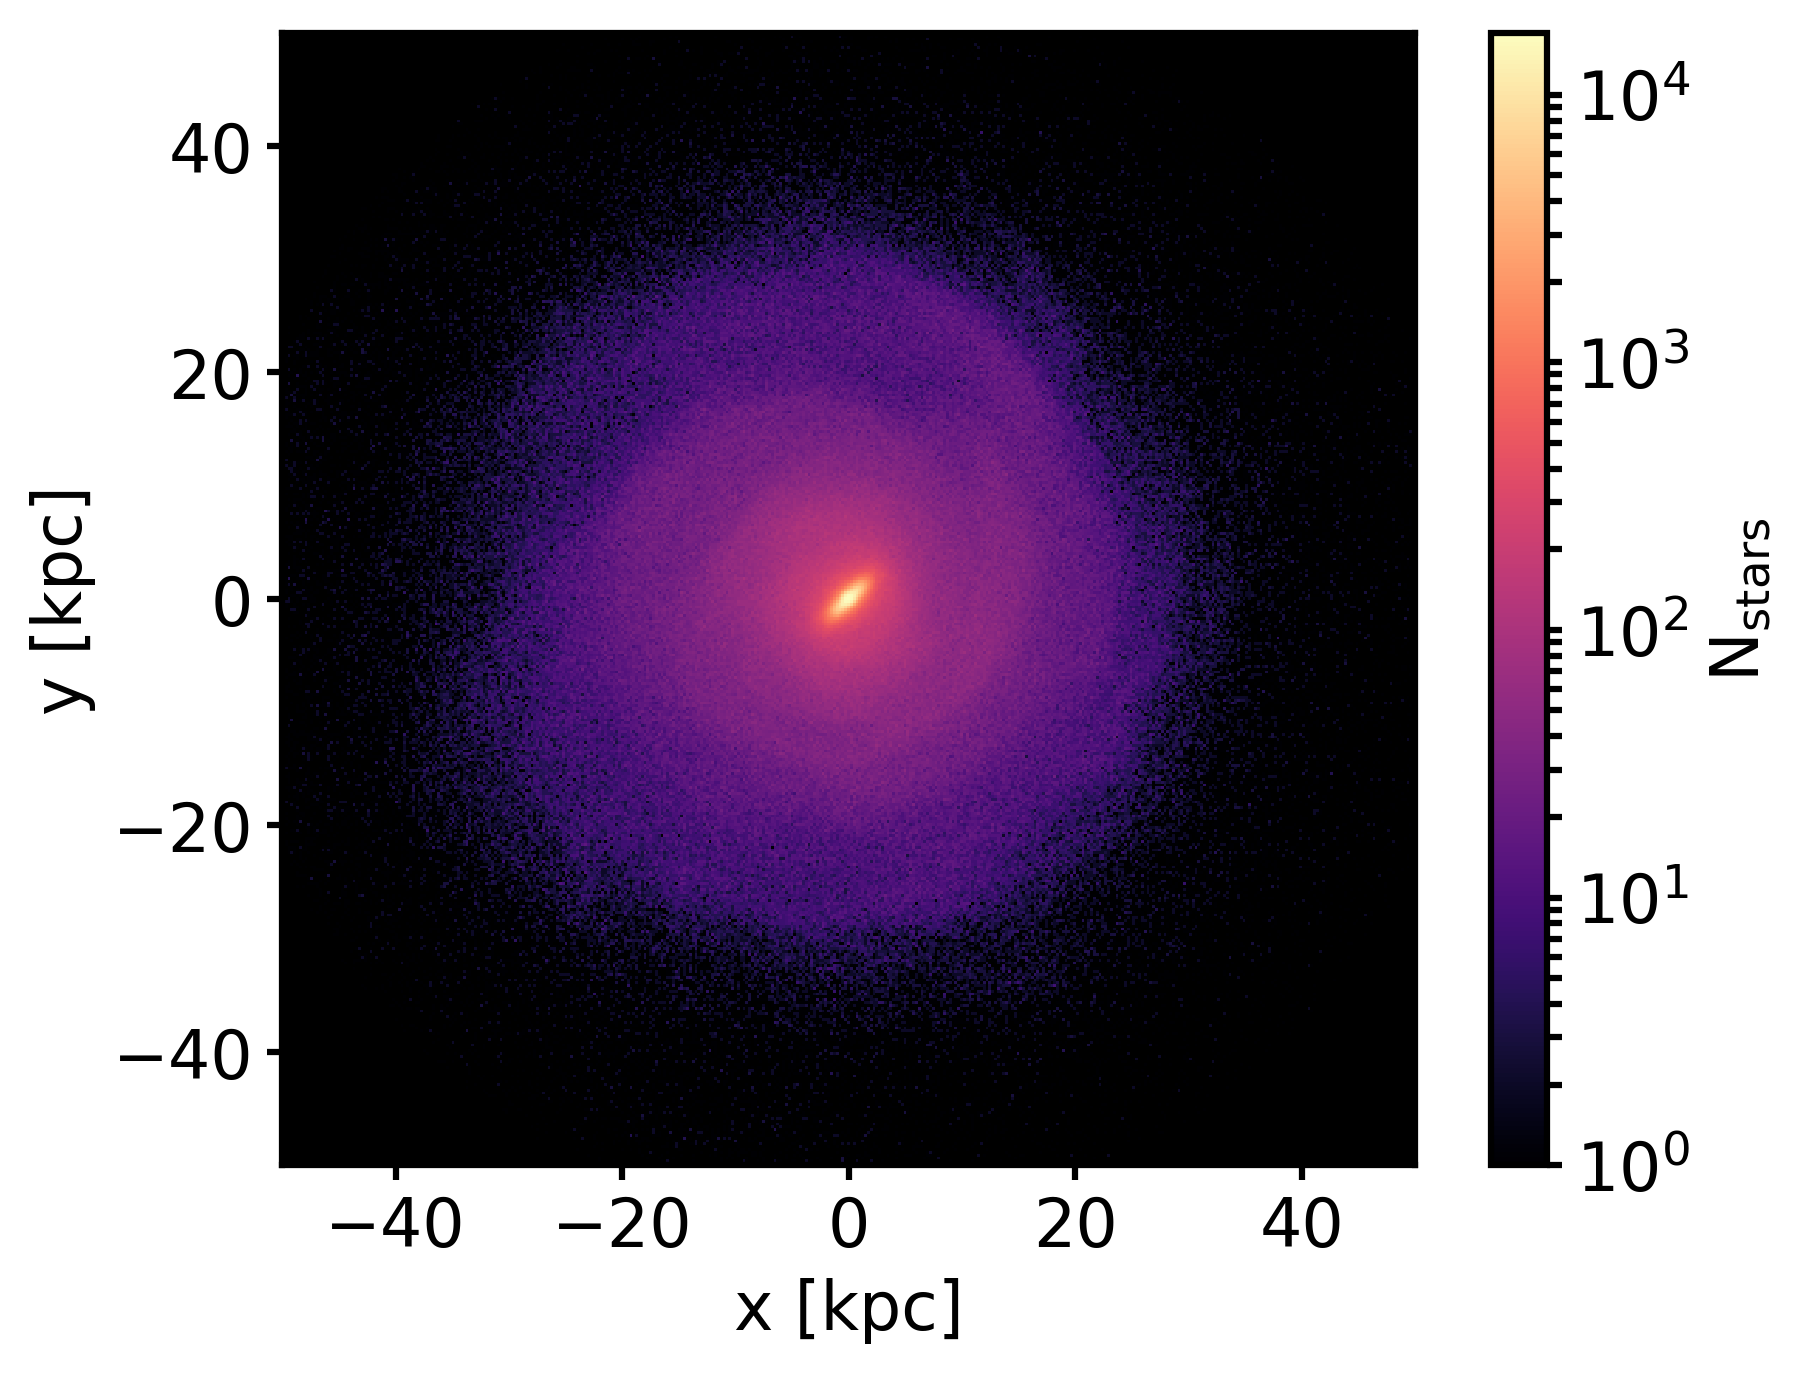
\includegraphics[width=\textwidth]{plots/Auriga/Au24_stars_xy_distribution_halo0_zoomin.png}
	    \label{fig:Au24_stars_xy_zoomin}
    \end{subfigure}
    
    \begin{subfigure}[b]{0.8\textwidth}
    \centering
    	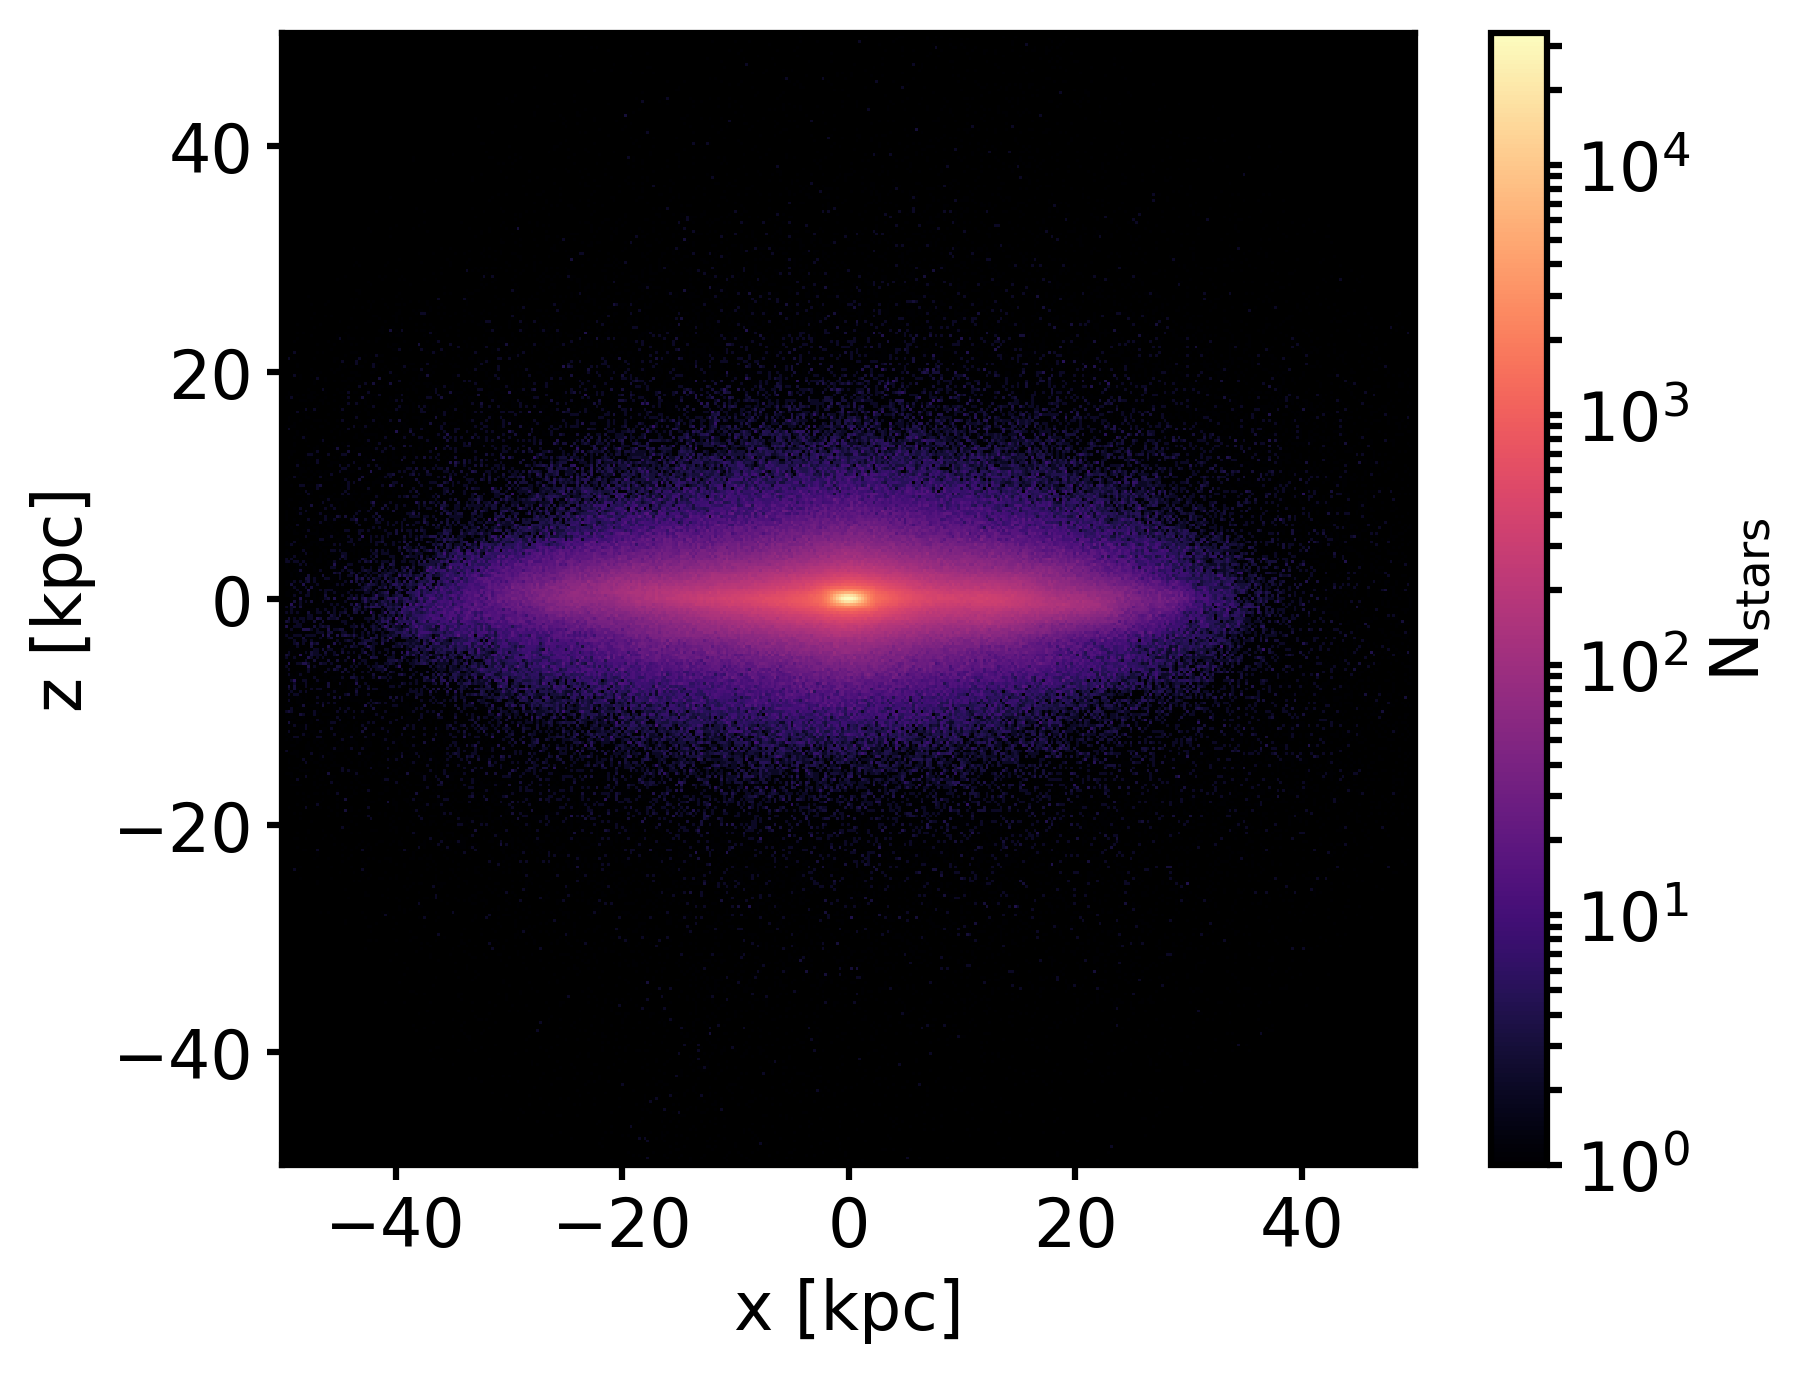
\includegraphics[width=\textwidth]{plots/Auriga/Au24_stars_xz_distribution_halo0_zoomin.png}
    	\label{fig:Au24_stars_xz_zoomin}
    \end{subfigure}
    \caption{Stellar distribution of main galaxy at $\textit{z}=0$.}\label{fig:Stars_AU24}
\end{figure}

\subsection{Best fit potential}
The best fit potential of a galaxy should be a analytic, axisymmetric potential so that we are able  to compare our results to the results of observers, since they mostly fit external galaxies in such a structure. We need to take into account that the galaxy evolved not isolated but went through many mergers and therefore its potential is either analytic nor axisymmetric but has a lot of substructure. The fit is only a vague approximation. Also it is self-consistent so changes in potential influence the velocities of the objects inside and changes on the positions of the objects will change the gravitational potential. Since we fit a potential to each snapshot we have a time-dependent potential. We also need to include a disk and bulge decomposition which is not natural in a cosmological simulation. As the gas evolves in cells, we cannot calculate its density easily. Therefore, we do not consider it in our potential fits. Since we want to recreate observers way of looking at galaxies we do not need to include gas as observers in e.g. \ac{MGE} fits \citep{MGE...Monnet, MGE...Emsellem} also only take stellar light into account. 

\subsubsection{Component decomposition}
To fit a potential to each component, we first need to decompose the different parts. We assume that all \ac{DM} particles belonging to the main galaxy make up its halo. The stellar particles belong to either the spheroid or the disk. We distinguish these components by the use of the circularity parameter 
\begin{equation}
    \epsilon = \frac{L_z}{L_{z,max}(E)}
\end{equation}
where $L_{z,max}(E)$ is the maximum angular momentum allowed for the orbital energy $E$. 
$\epsilon = 1$ is a prograde circular orbit in the disc plane. $\epsilon = -1$ is a retrograde circular orbit in the disc plane. $\epsilon \sim 0$ is an orbit with a very low $z$-component of angular momentum which may be highly inclined to the disc spin axis and/or be highly eccentric.  

\cite{AurigaGrand} uses two different methods two distinguish the components:
\begin{enumerate}
\item Mirror negative $\epsilon$ as bulge material, the rest belongs to the disk.
\item All particles with $\epsilon > 0.7$ are assigned to the disk.
\end{enumerate}

We use the second method. 


\\figure: Decomposition of stellar disk and spheroid using the circularity

\subsubsection{Disk potential}
We fit the disk with a \citet{MNprofile} potential following the profile 
\begin{equation}
\Phi(R,z) = -\frac{GM}{\sqrt{R^2+(a+\sqrt{z^2+b^2})^2}}
\end{equation} 
with scale length $a$ and scale height $b$ which provides a disk with a finite thickness. If $b\rightarrow 0$, the disk will be infinite thin and if $a \rightarrow 0$ the potential has a spherical density distribution. $b/a$ therefore defines the flattening of the system. It is a rather simply model with only a small computational costs. Therefore it is widely used. It has limitations in the mid-plane ($z=0$) at high $R$. 

\begin{figure}
    \centering
    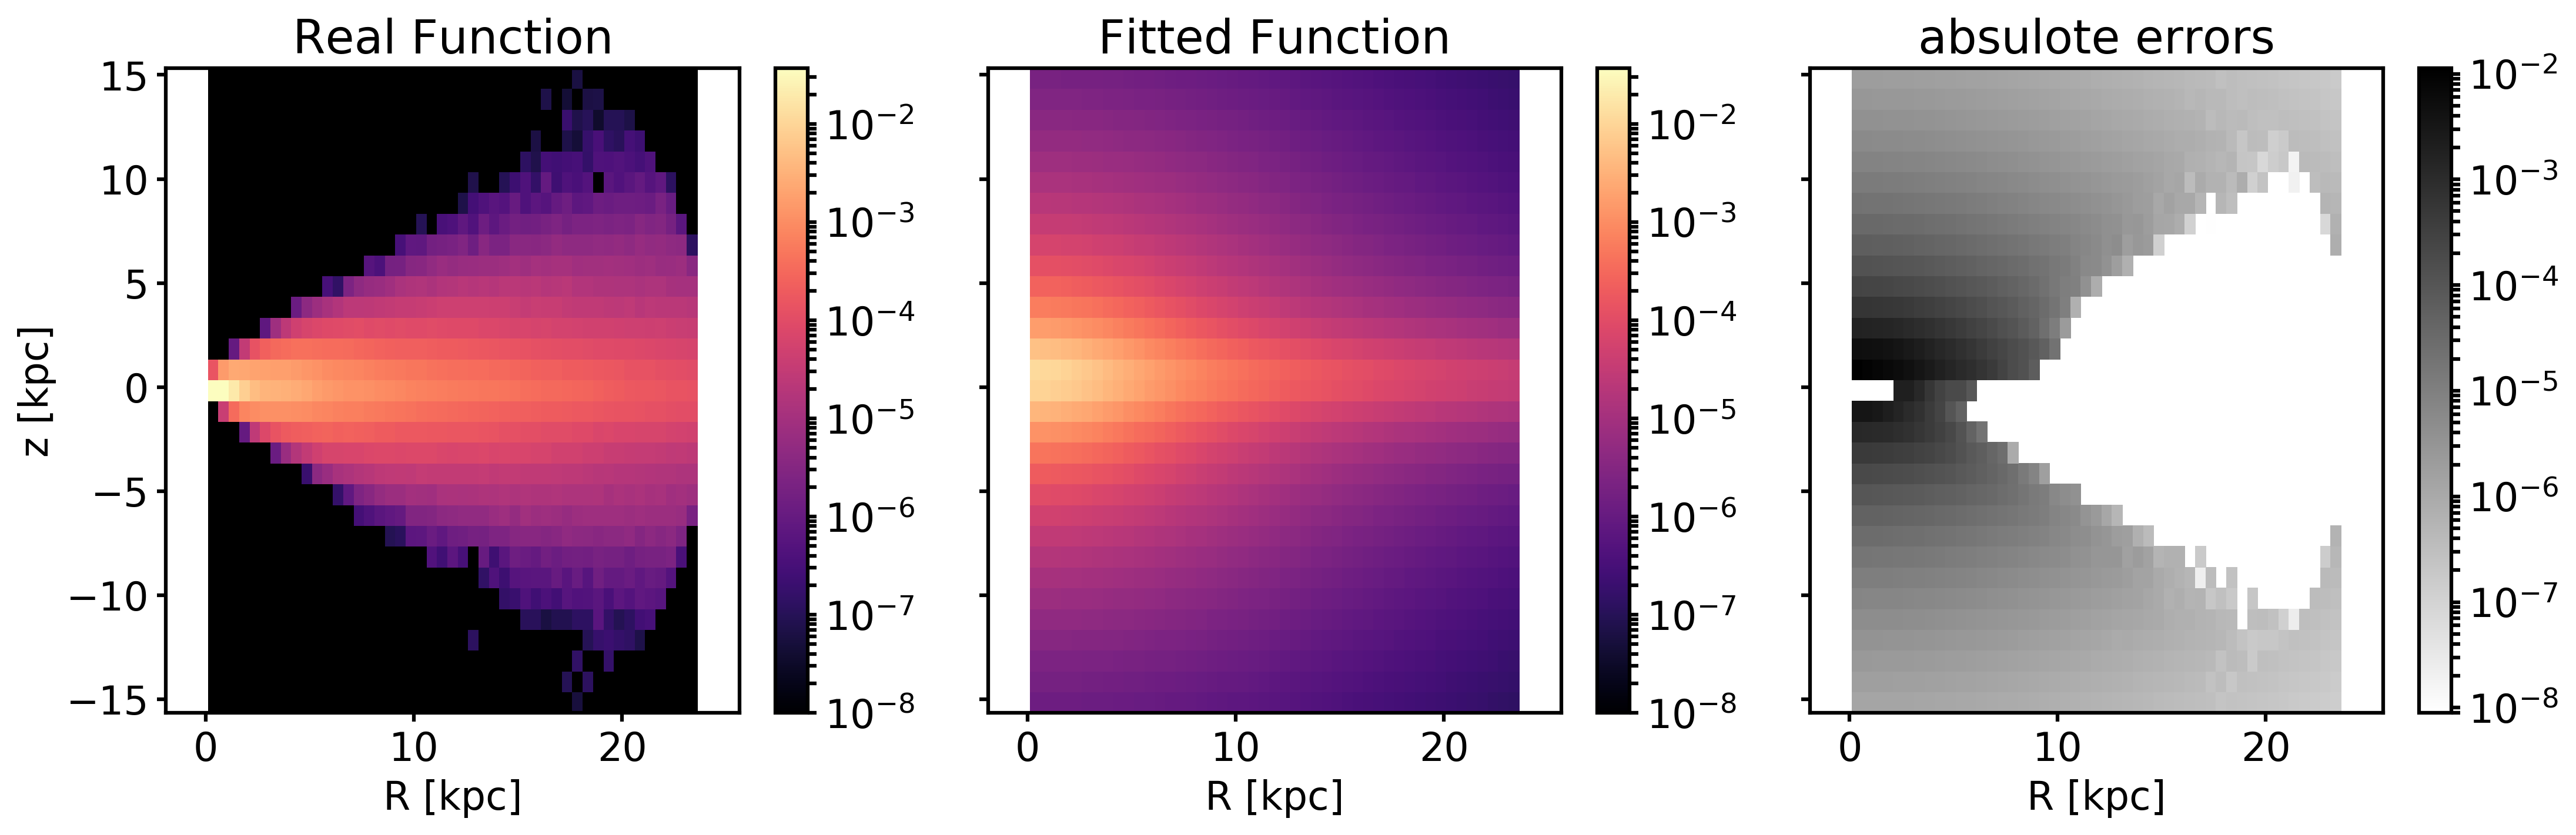
\includegraphics[width = \textwidth]{plots/Auriga/MND_best_fit.png}
    \caption{2d density of MN disk data + best fit + absolute difference.}
    \label{fig:MND}
\end{figure}

\subsubsection{Spheroid potential}\label{subsec:spher_pot}
For the central stellar spheroid, we apply a \citet{Hernquistprofile} potential which has the density 
\begin{equation}
    \rho = \frac{M}{2\pi}\frac{a}{r}\frac{1}{(r+a)^3}
\end{equation}
where $M$ is the total stellar mass and $a$ is the scale length. 





\subsubsection{Halo Potential}
We model the \ac{DM} halo with a \citet{NFWprofile} profile following the formula 
\begin{equation}
    \frac{\rho(r)}{\rho_{crit}} = \frac{\delta_c}{(r/r_s)(1+r/r_s)^2}
\end{equation} with the critical density $\rho_{crit} = 3H^2 / 8\pi G $, scale radius $r_s$  and a characteristic and dimensionless density $\delta_c$. 






\subsubsection{Total potential}
\begin{figure}
    \centering
    \begin{subfigure}[b]{0.3\textwidth}
	    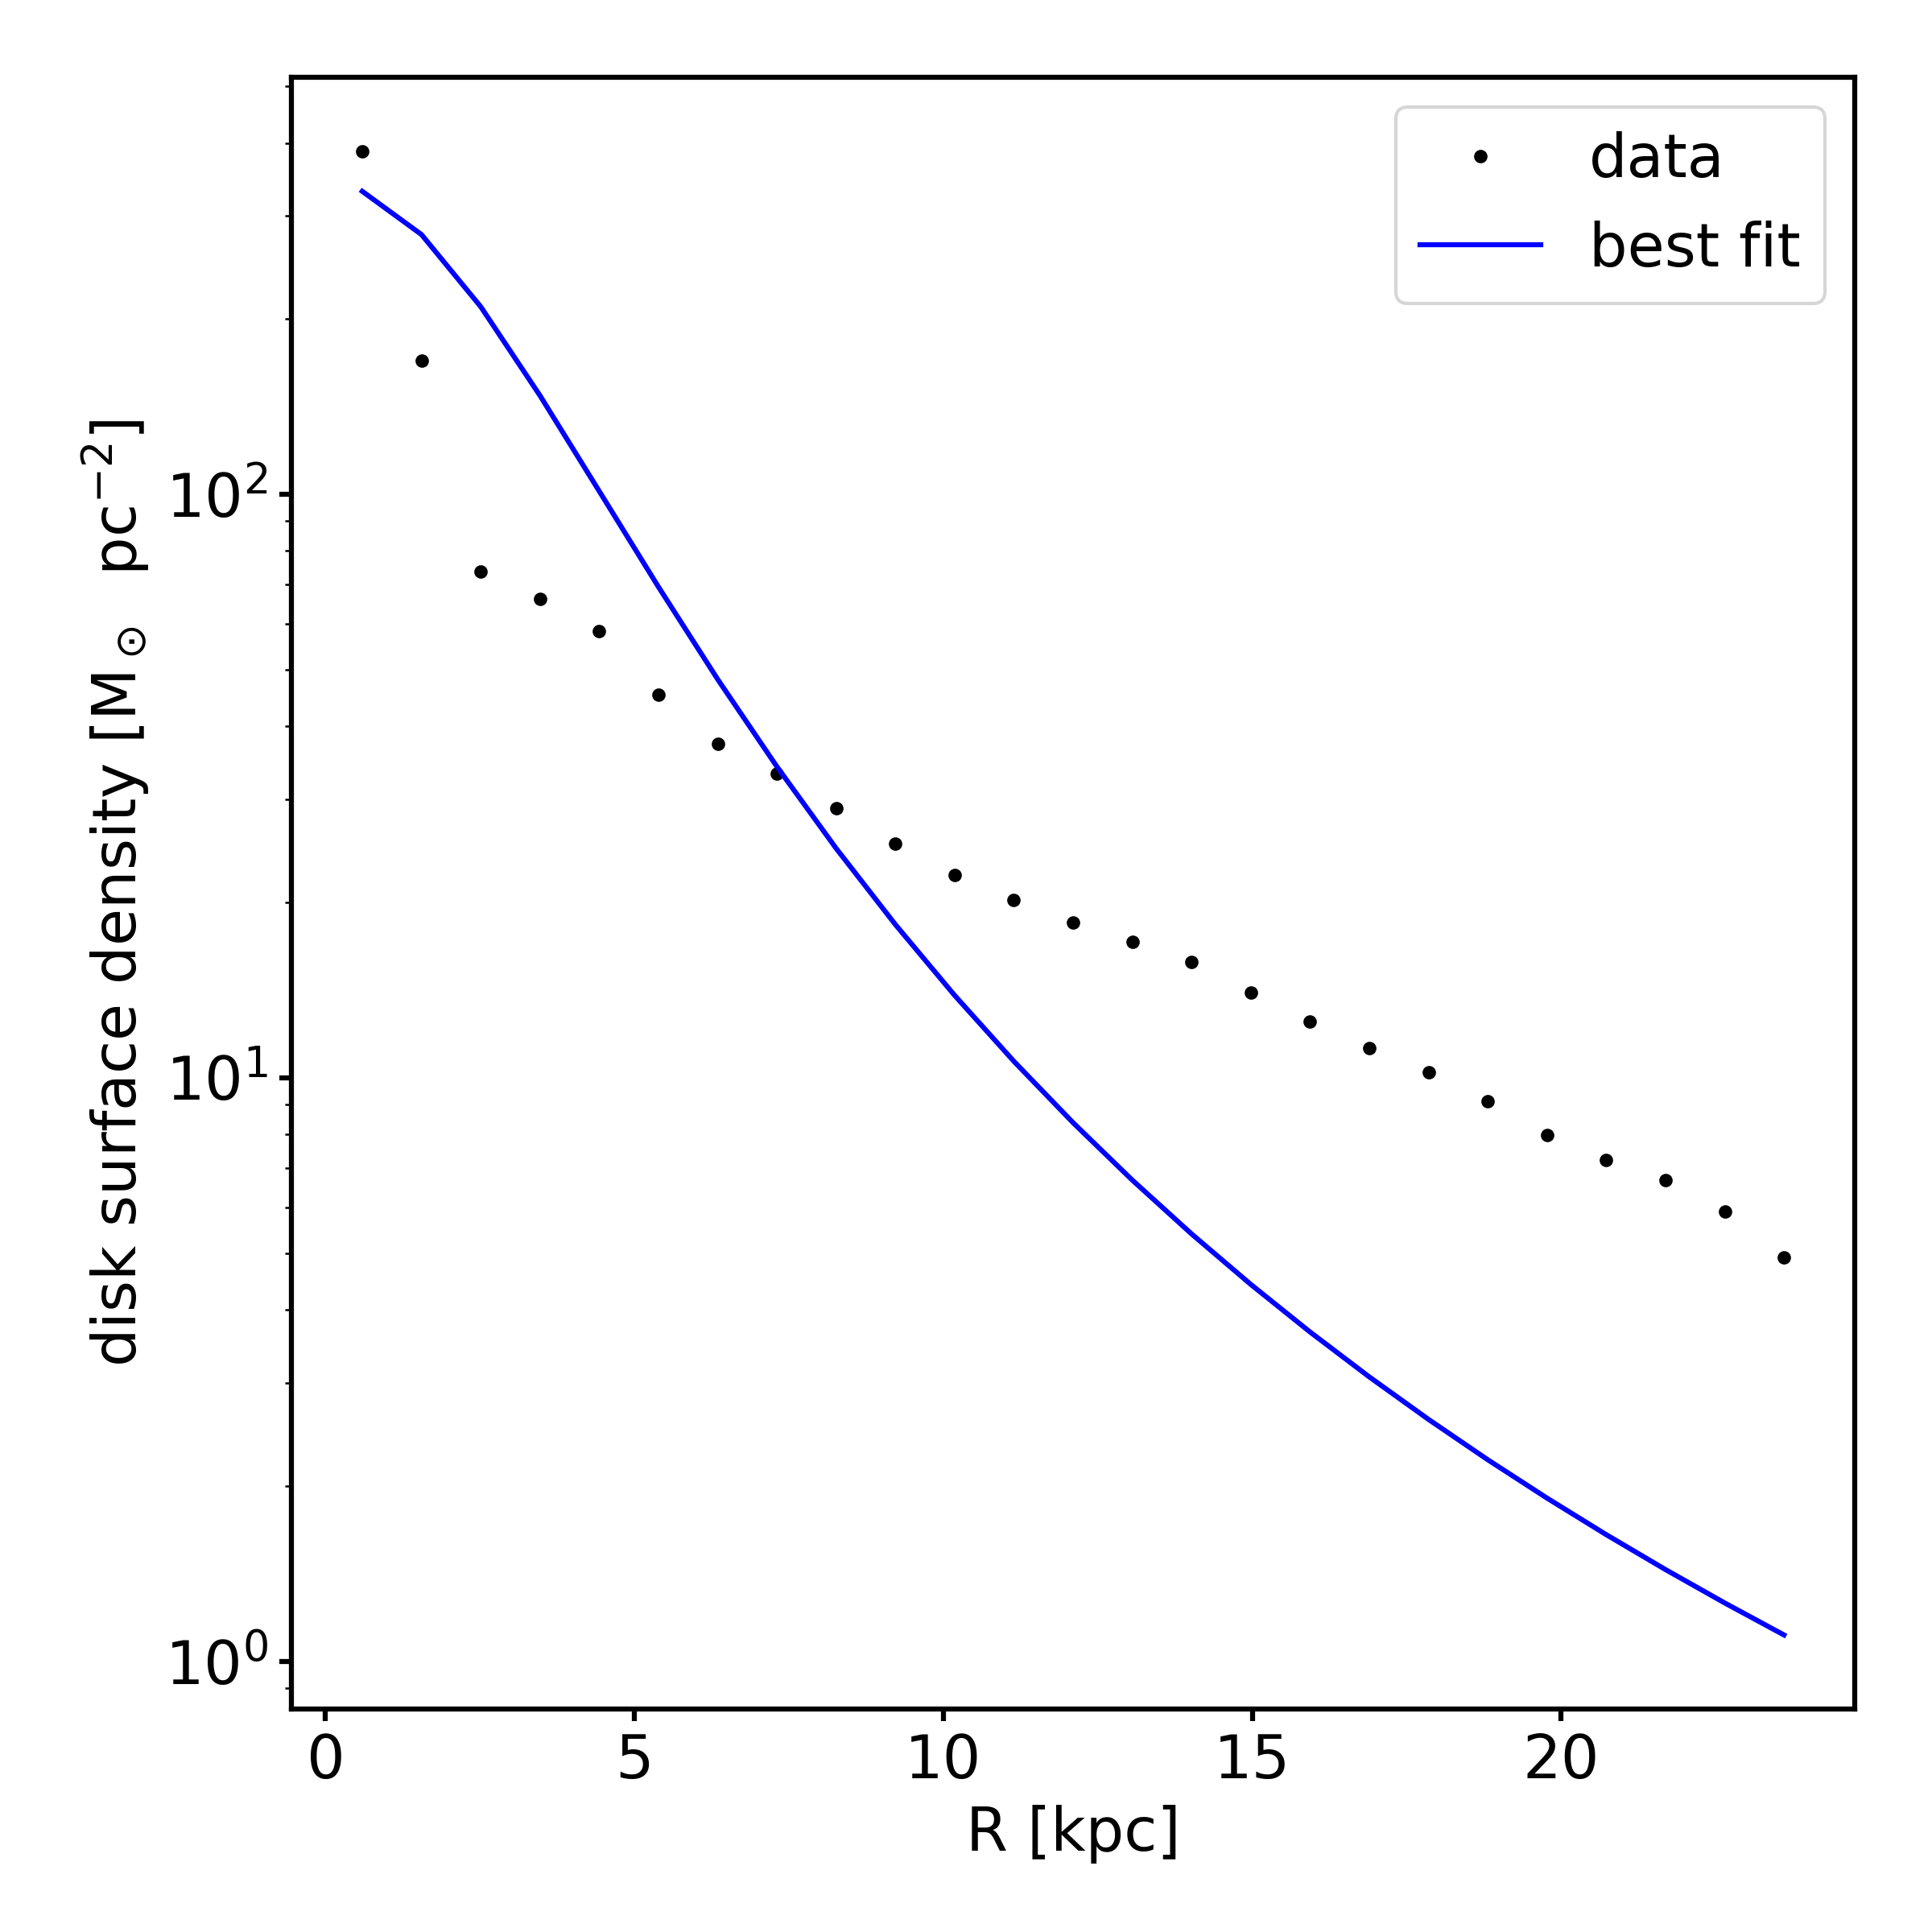
\includegraphics[width=\textwidth]{plots/Auriga/surface_dens_disk_fit_data.png}
	    \label{fig:disk_surfdens_fit}
    \end{subfigure}
    ~ %add desired spacing between images, e. g. ~, \quad, \qquad, \hfill etc. 
      %(or a blank line to force the subfigure onto a new line)
    \begin{subfigure}[b]{0.3\textwidth}
    \centering
    	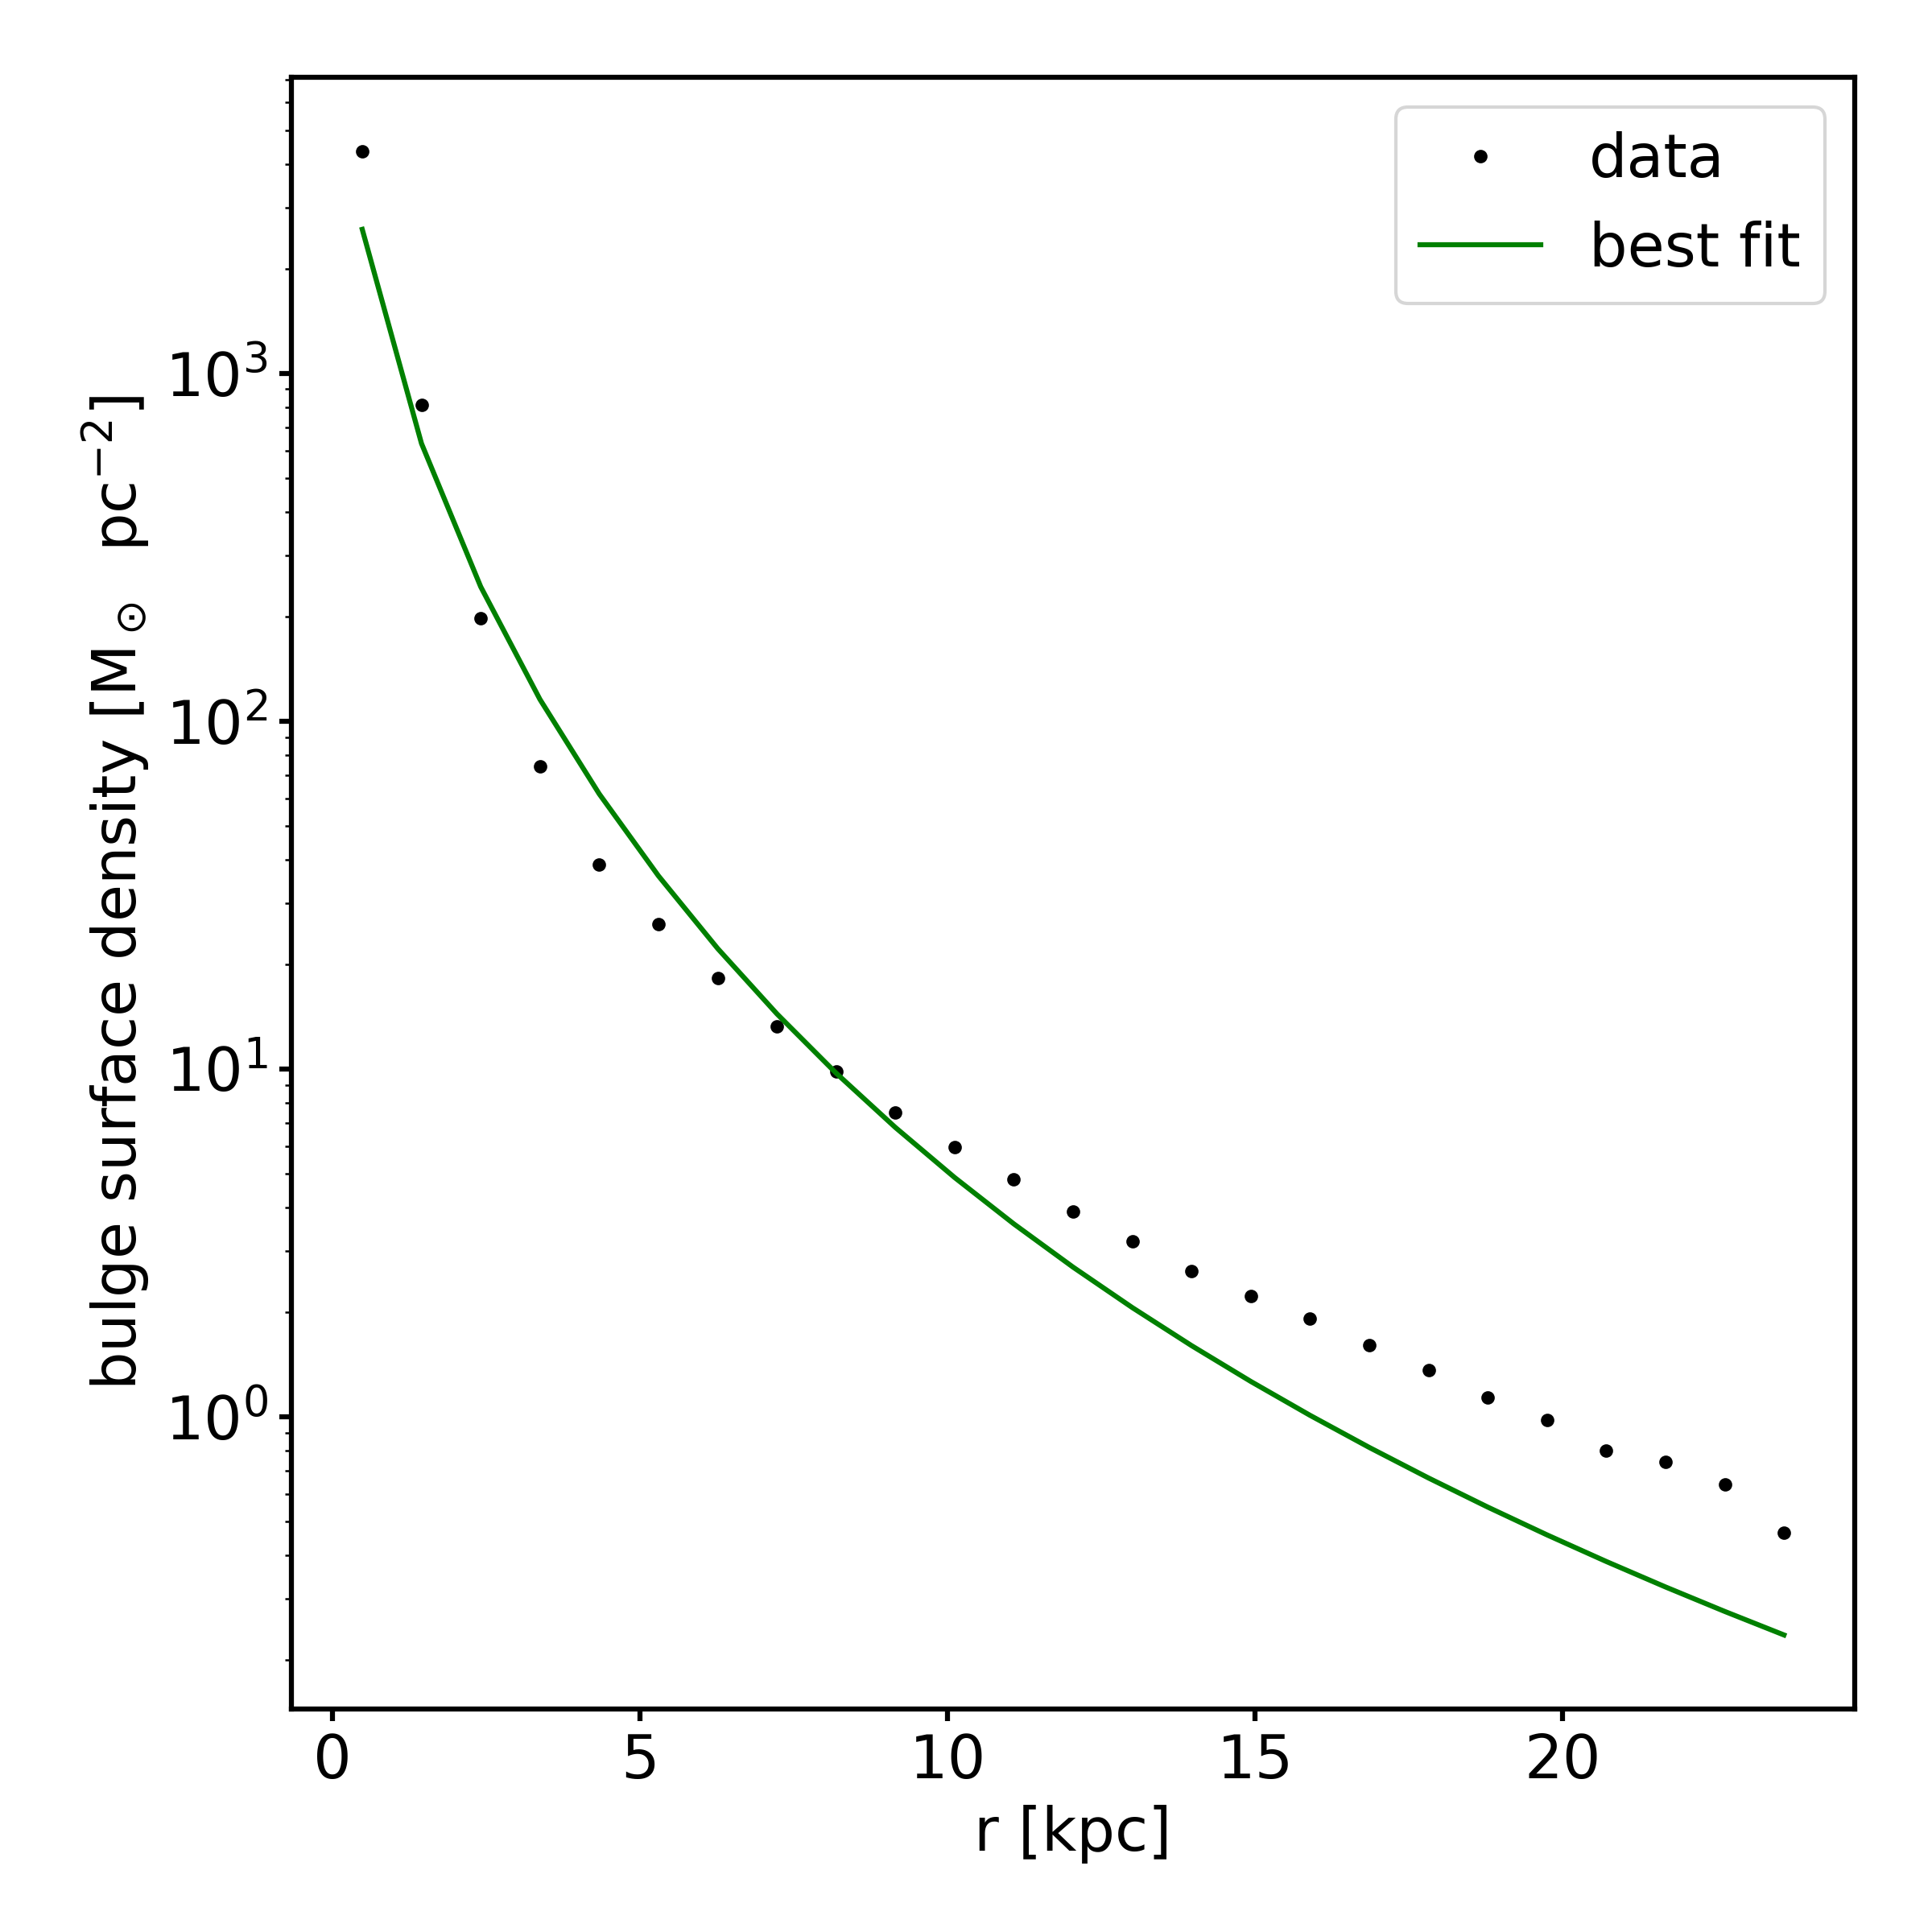
\includegraphics[width=\textwidth]{plots/Auriga/surface_dens_spher_fit_data.png}
    	\label{fig:spher_surfdens_fit}
    \end{subfigure}
    ~ %add desired spacing between images, e. g. ~, \quad, \qquad, \hfill etc. 
    %(or a blank line to force the subfigure onto a new line)
    \begin{subfigure}[b]{0.3\textwidth}
    \centering
    	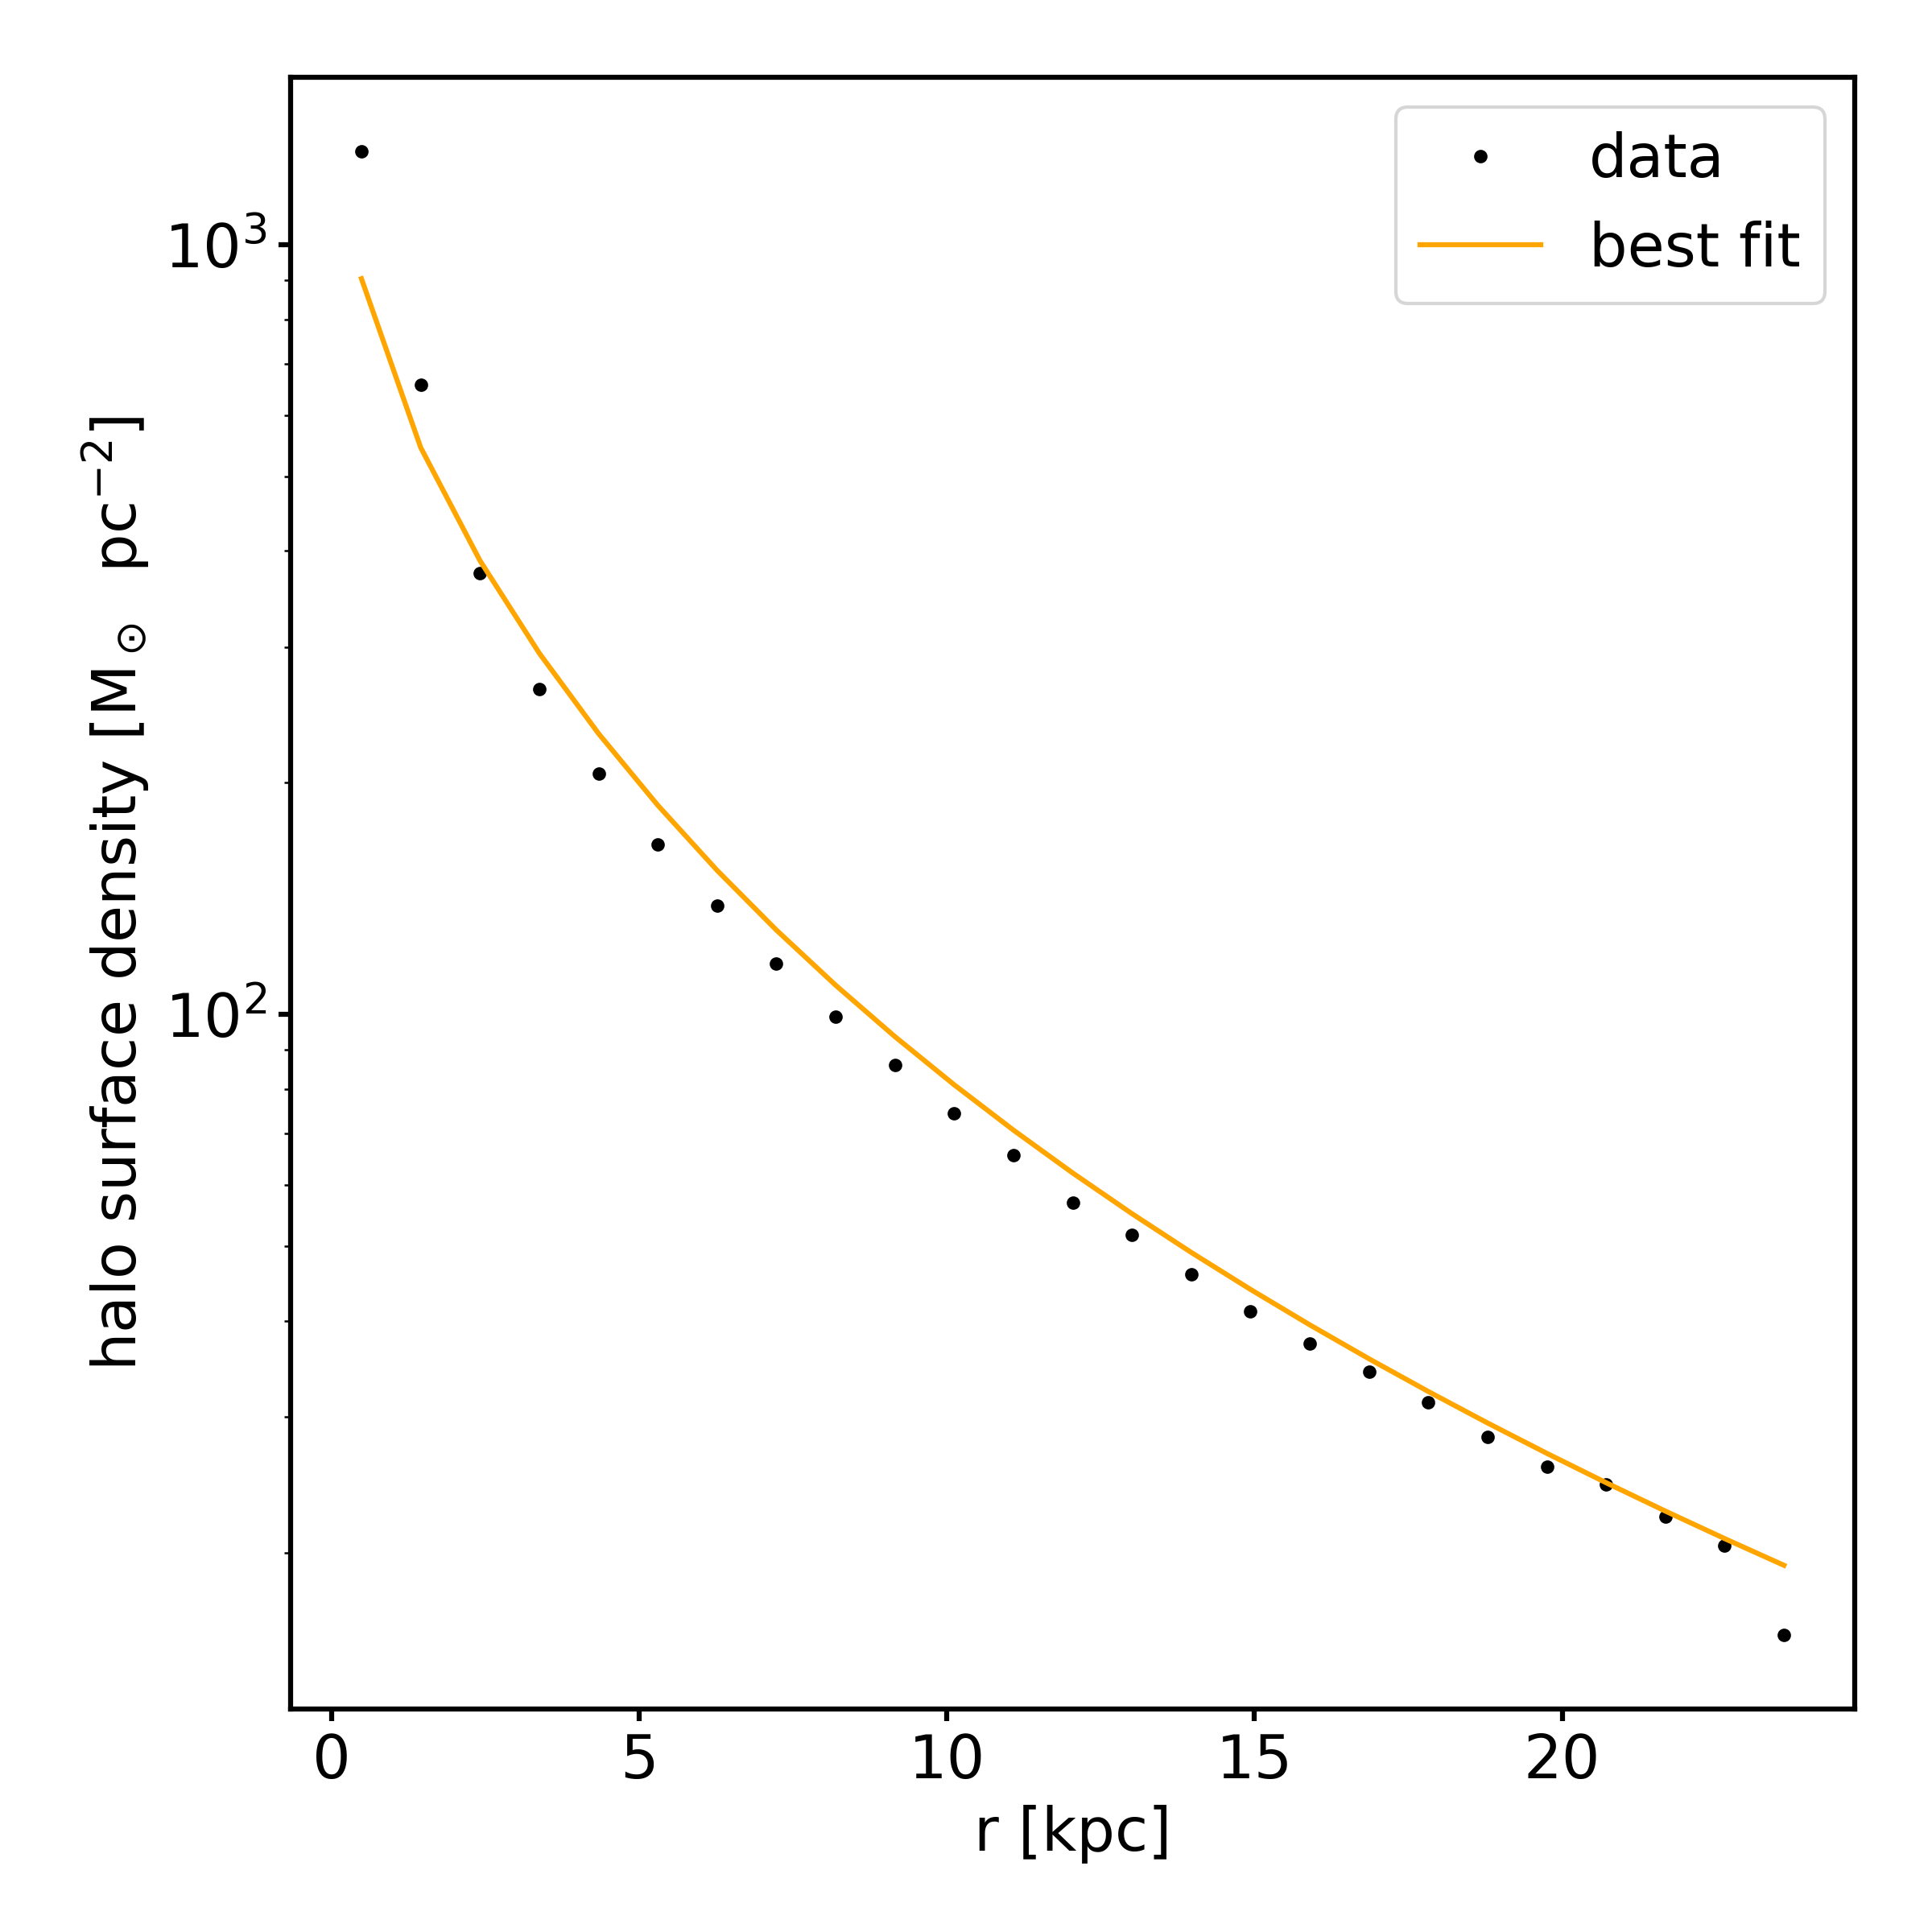
\includegraphics[width=\textwidth]{plots/Auriga/surface_dens_halo_fit_data.png}
    	\label{fig:halo_surfdens_fit}
    \end{subfigure}
    
    \begin{subfigure}[b]{0.3\textwidth}
        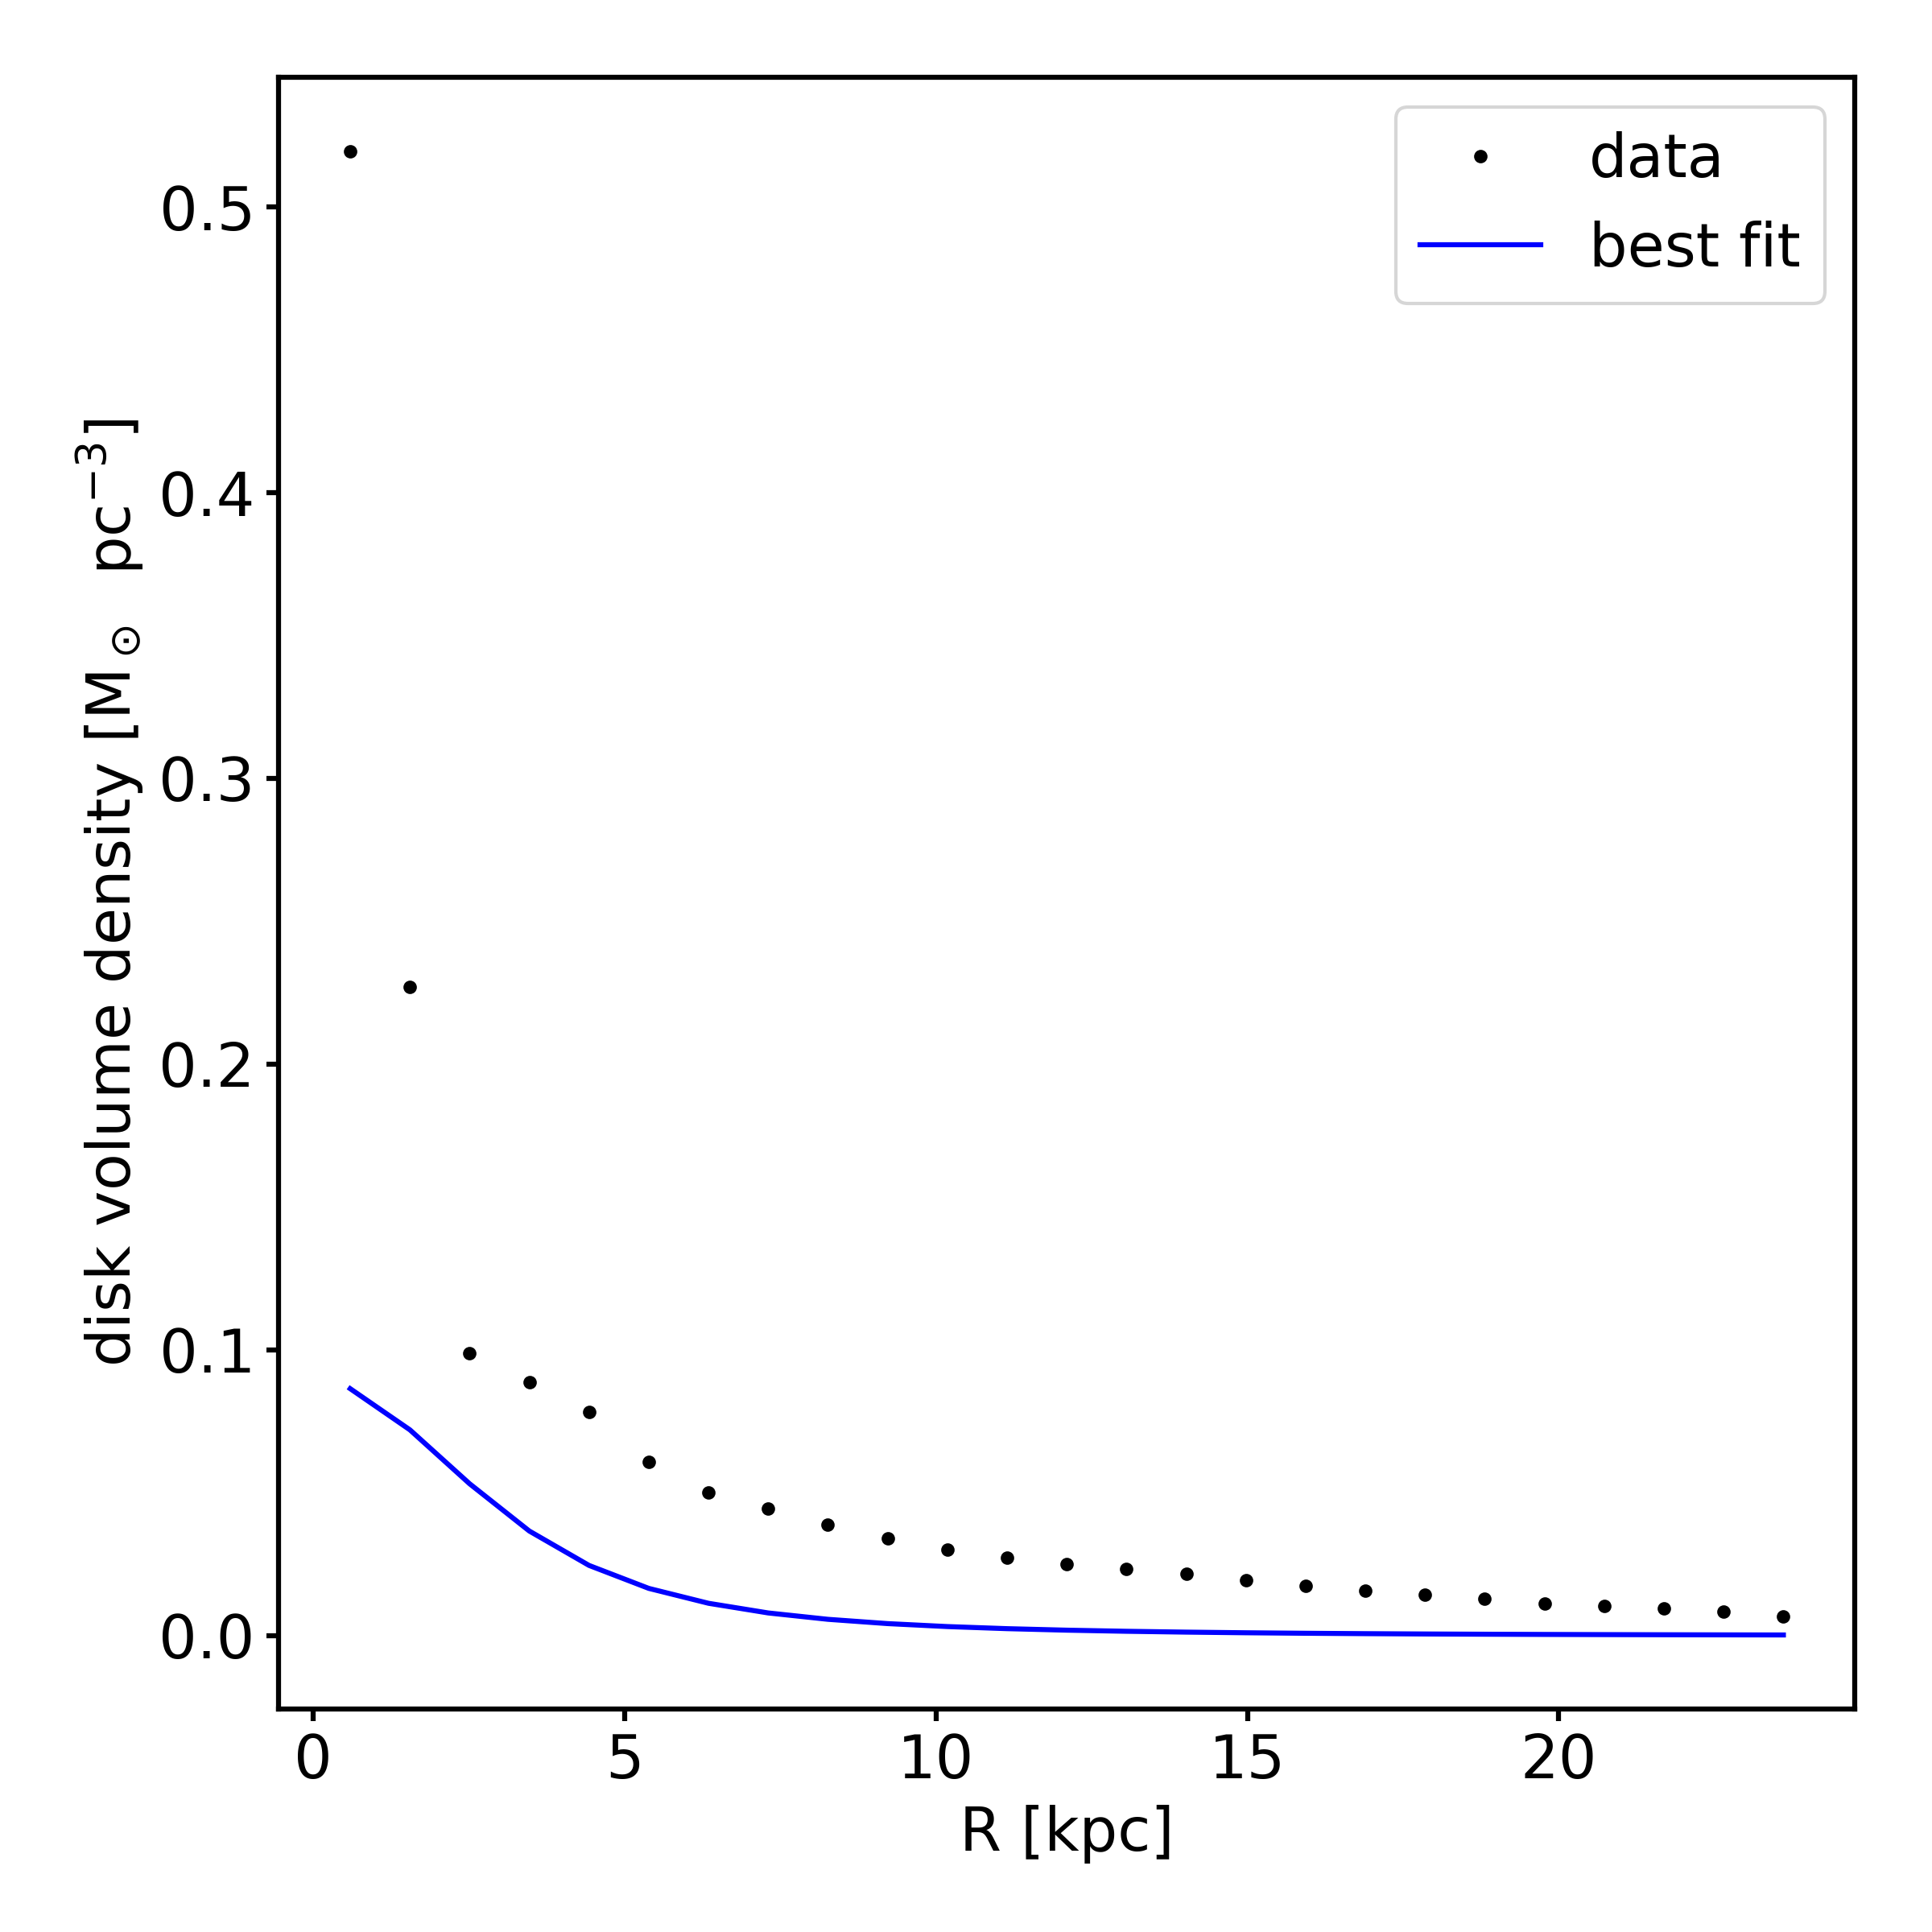
\includegraphics[width=\textwidth]{plots/Auriga/volume_dens_disk_fit_data.png}
	    \label{fig:disk_voldens_fit}
    \end{subfigure}
    ~ %add desired spacing between images, e. g. ~, \quad, \qquad, \hfill etc. 
    %(or a blank line to force the subfigure onto a new line)
    \begin{subfigure}[b]{0.3\textwidth}
    \centering
    	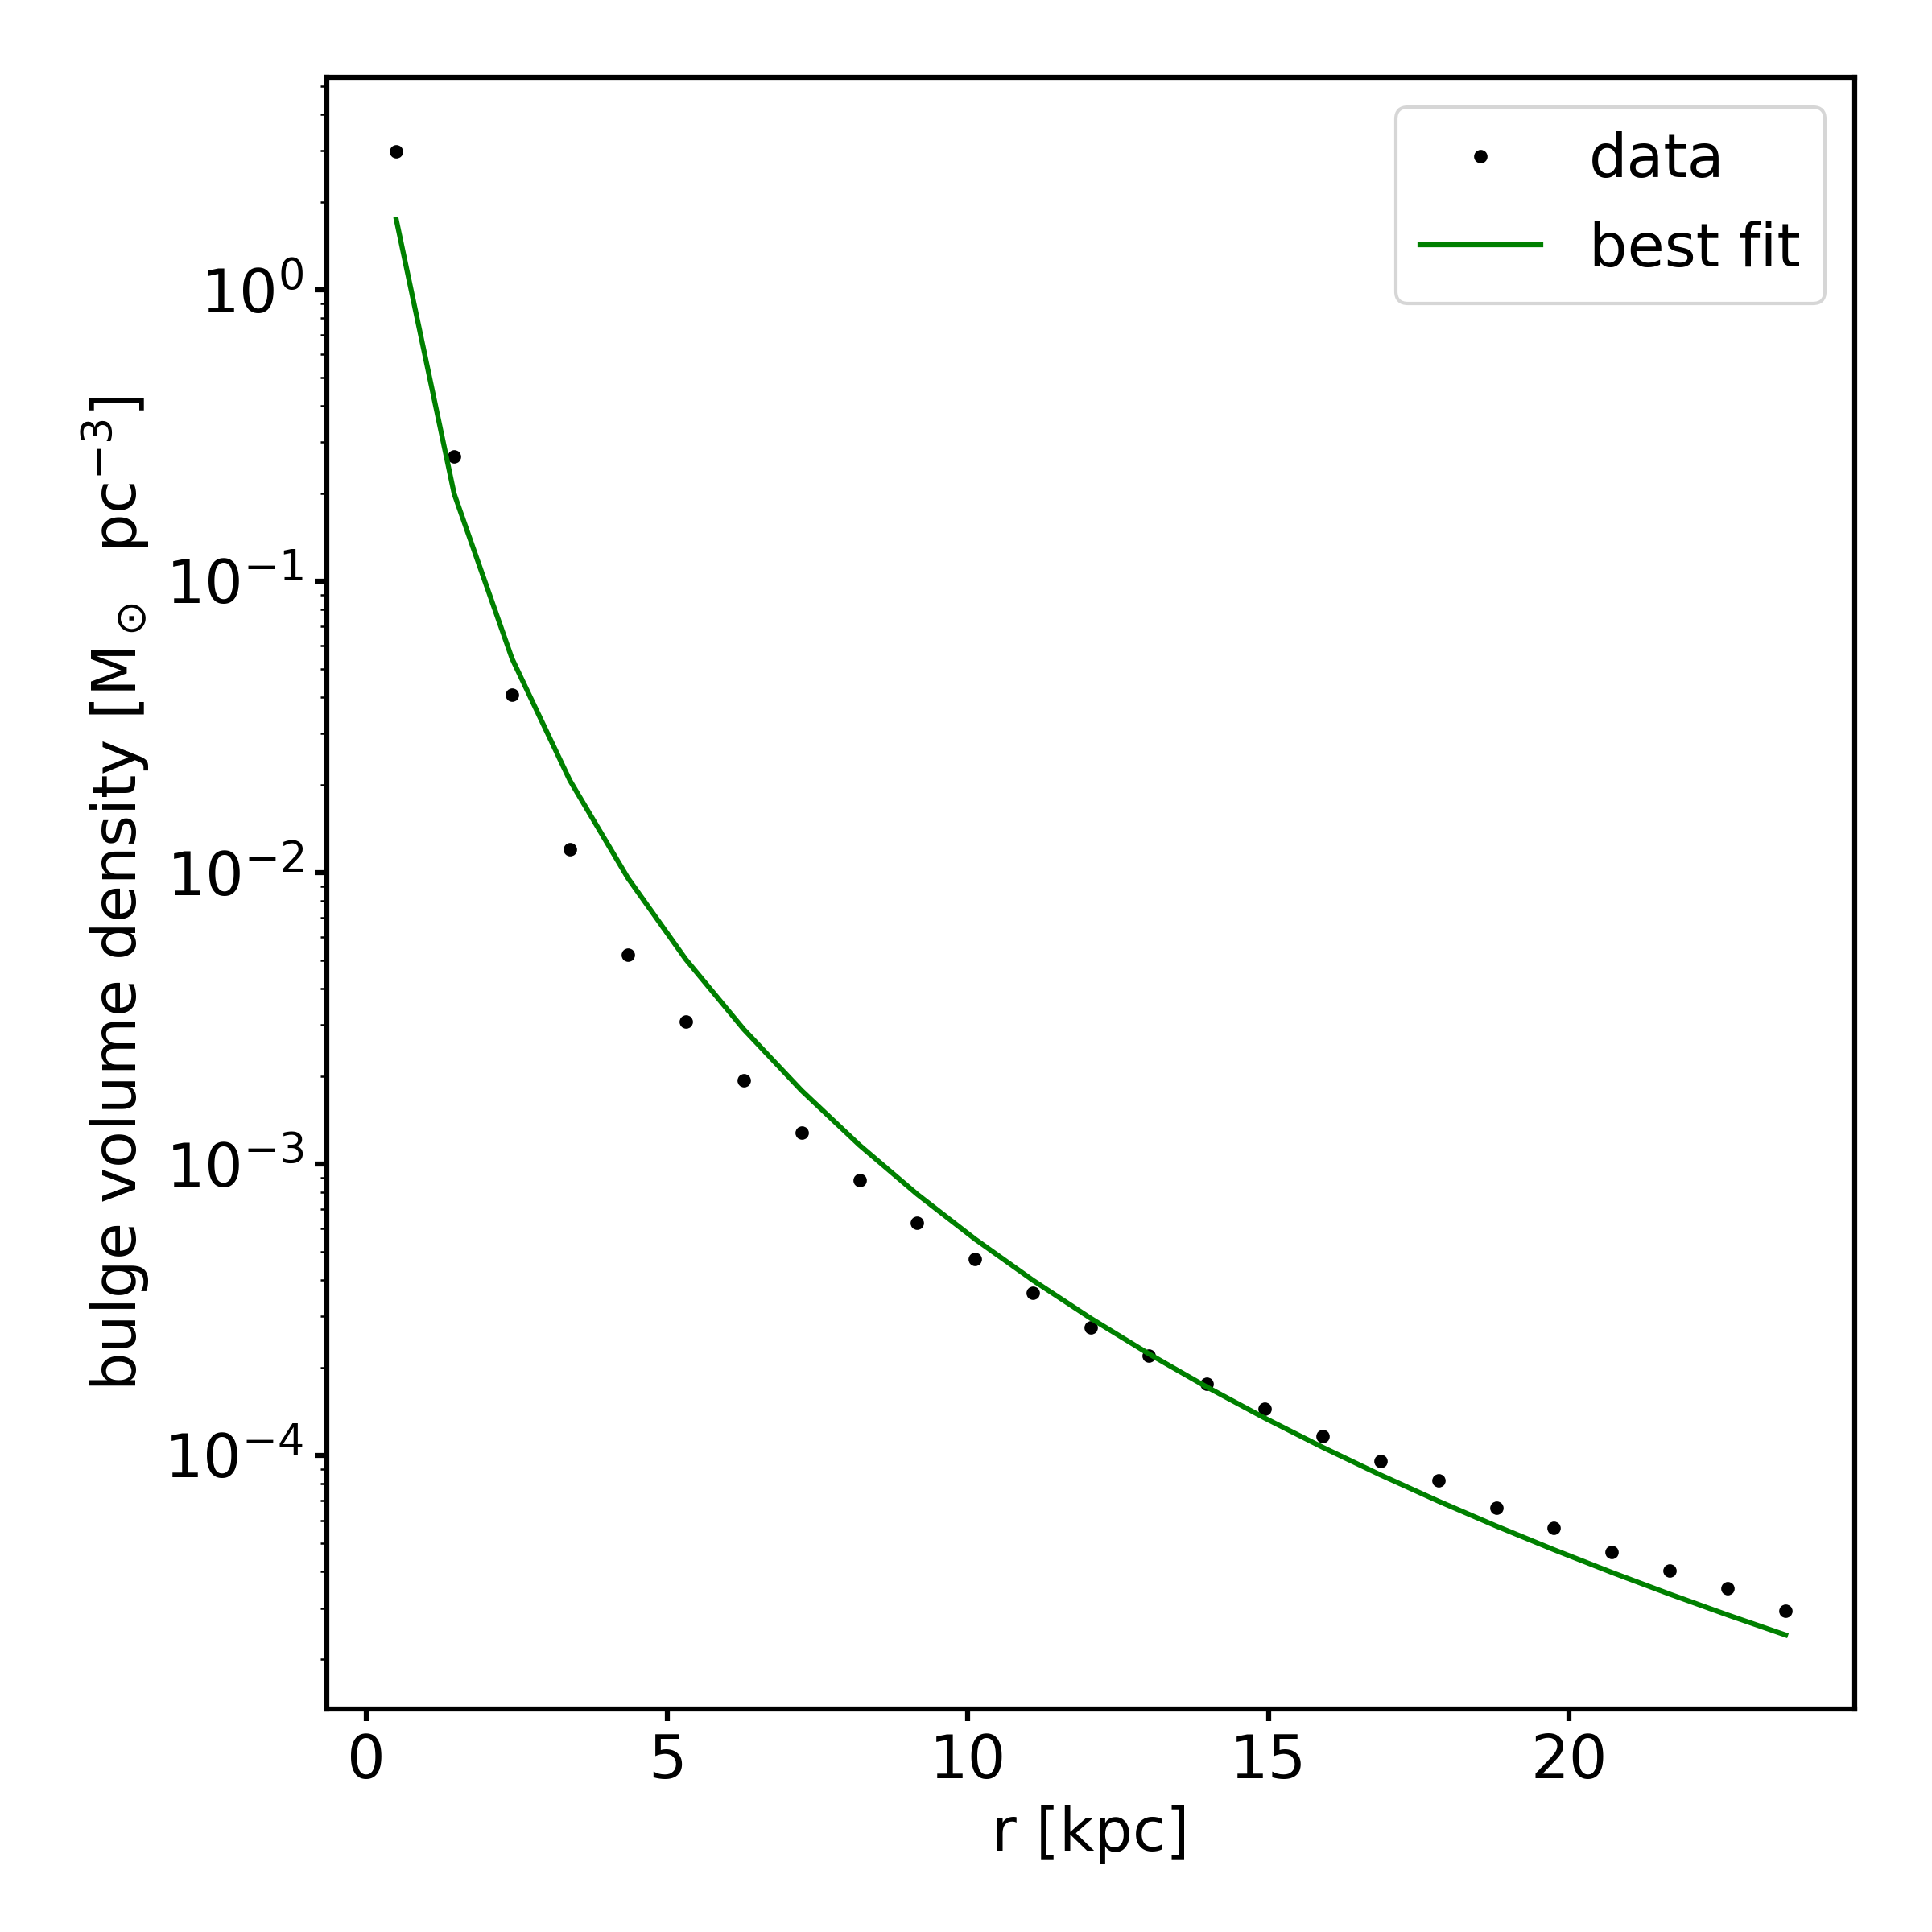
\includegraphics[width=\textwidth]{plots/Auriga/volume_dens_bulge_fit_data.png}
    	\label{fig:spher_voldens_fit}
    \end{subfigure}
    ~ %add desired spacing between images, e. g. ~, \quad, \qquad, \hfill etc. 
    %(or a blank line to force the subfigure onto a new line)
    \begin{subfigure}[b]{0.3\textwidth}
        \centering
    	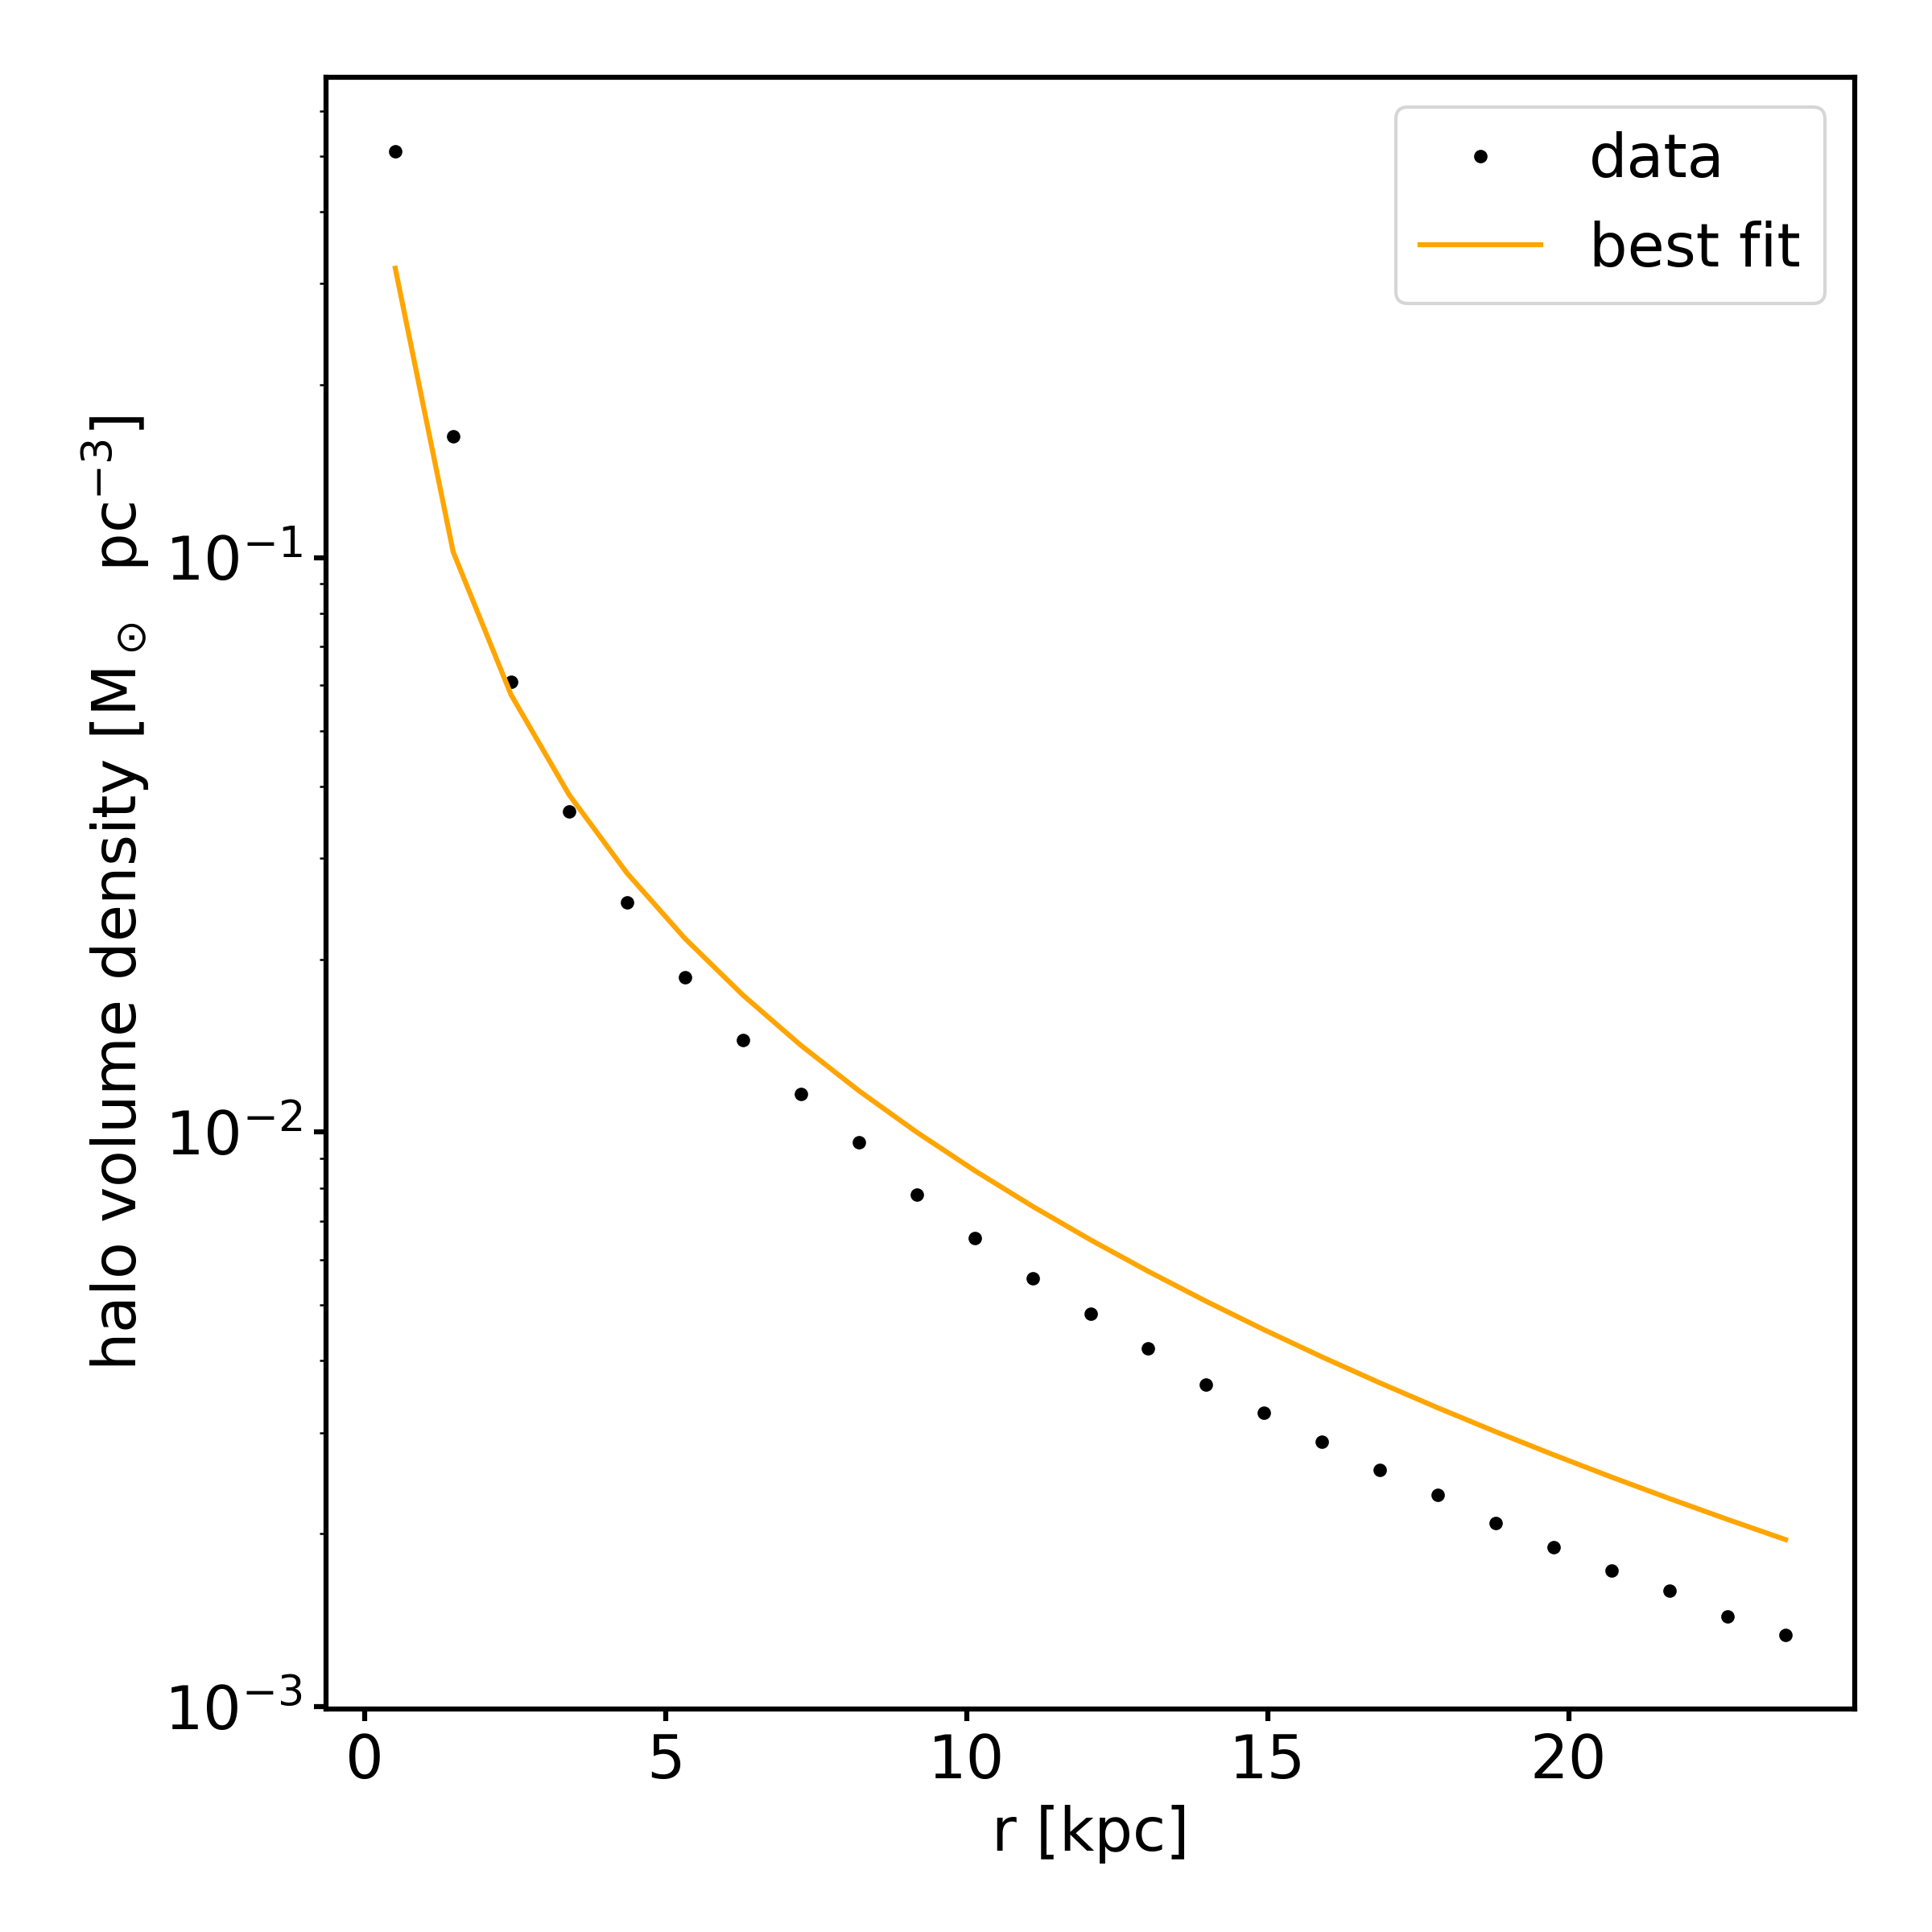
\includegraphics[width=\textwidth]{plots/Auriga/volume_dens_halo_fit_data.png}
	    \label{fig:halo_voldens_fit}
    \end{subfigure}
    \caption{Surface densities (upper row) and mass densities (lower row) of the components and their best fits at $\textit{z}=0$. Left (blue): stellar disk, middle (green): stellar spheroid, right (yellow): \ac{DM} halo.}\label{fig:single_pot_fits}
\end{figure}

\begin{figure}[htbp]
\centering
	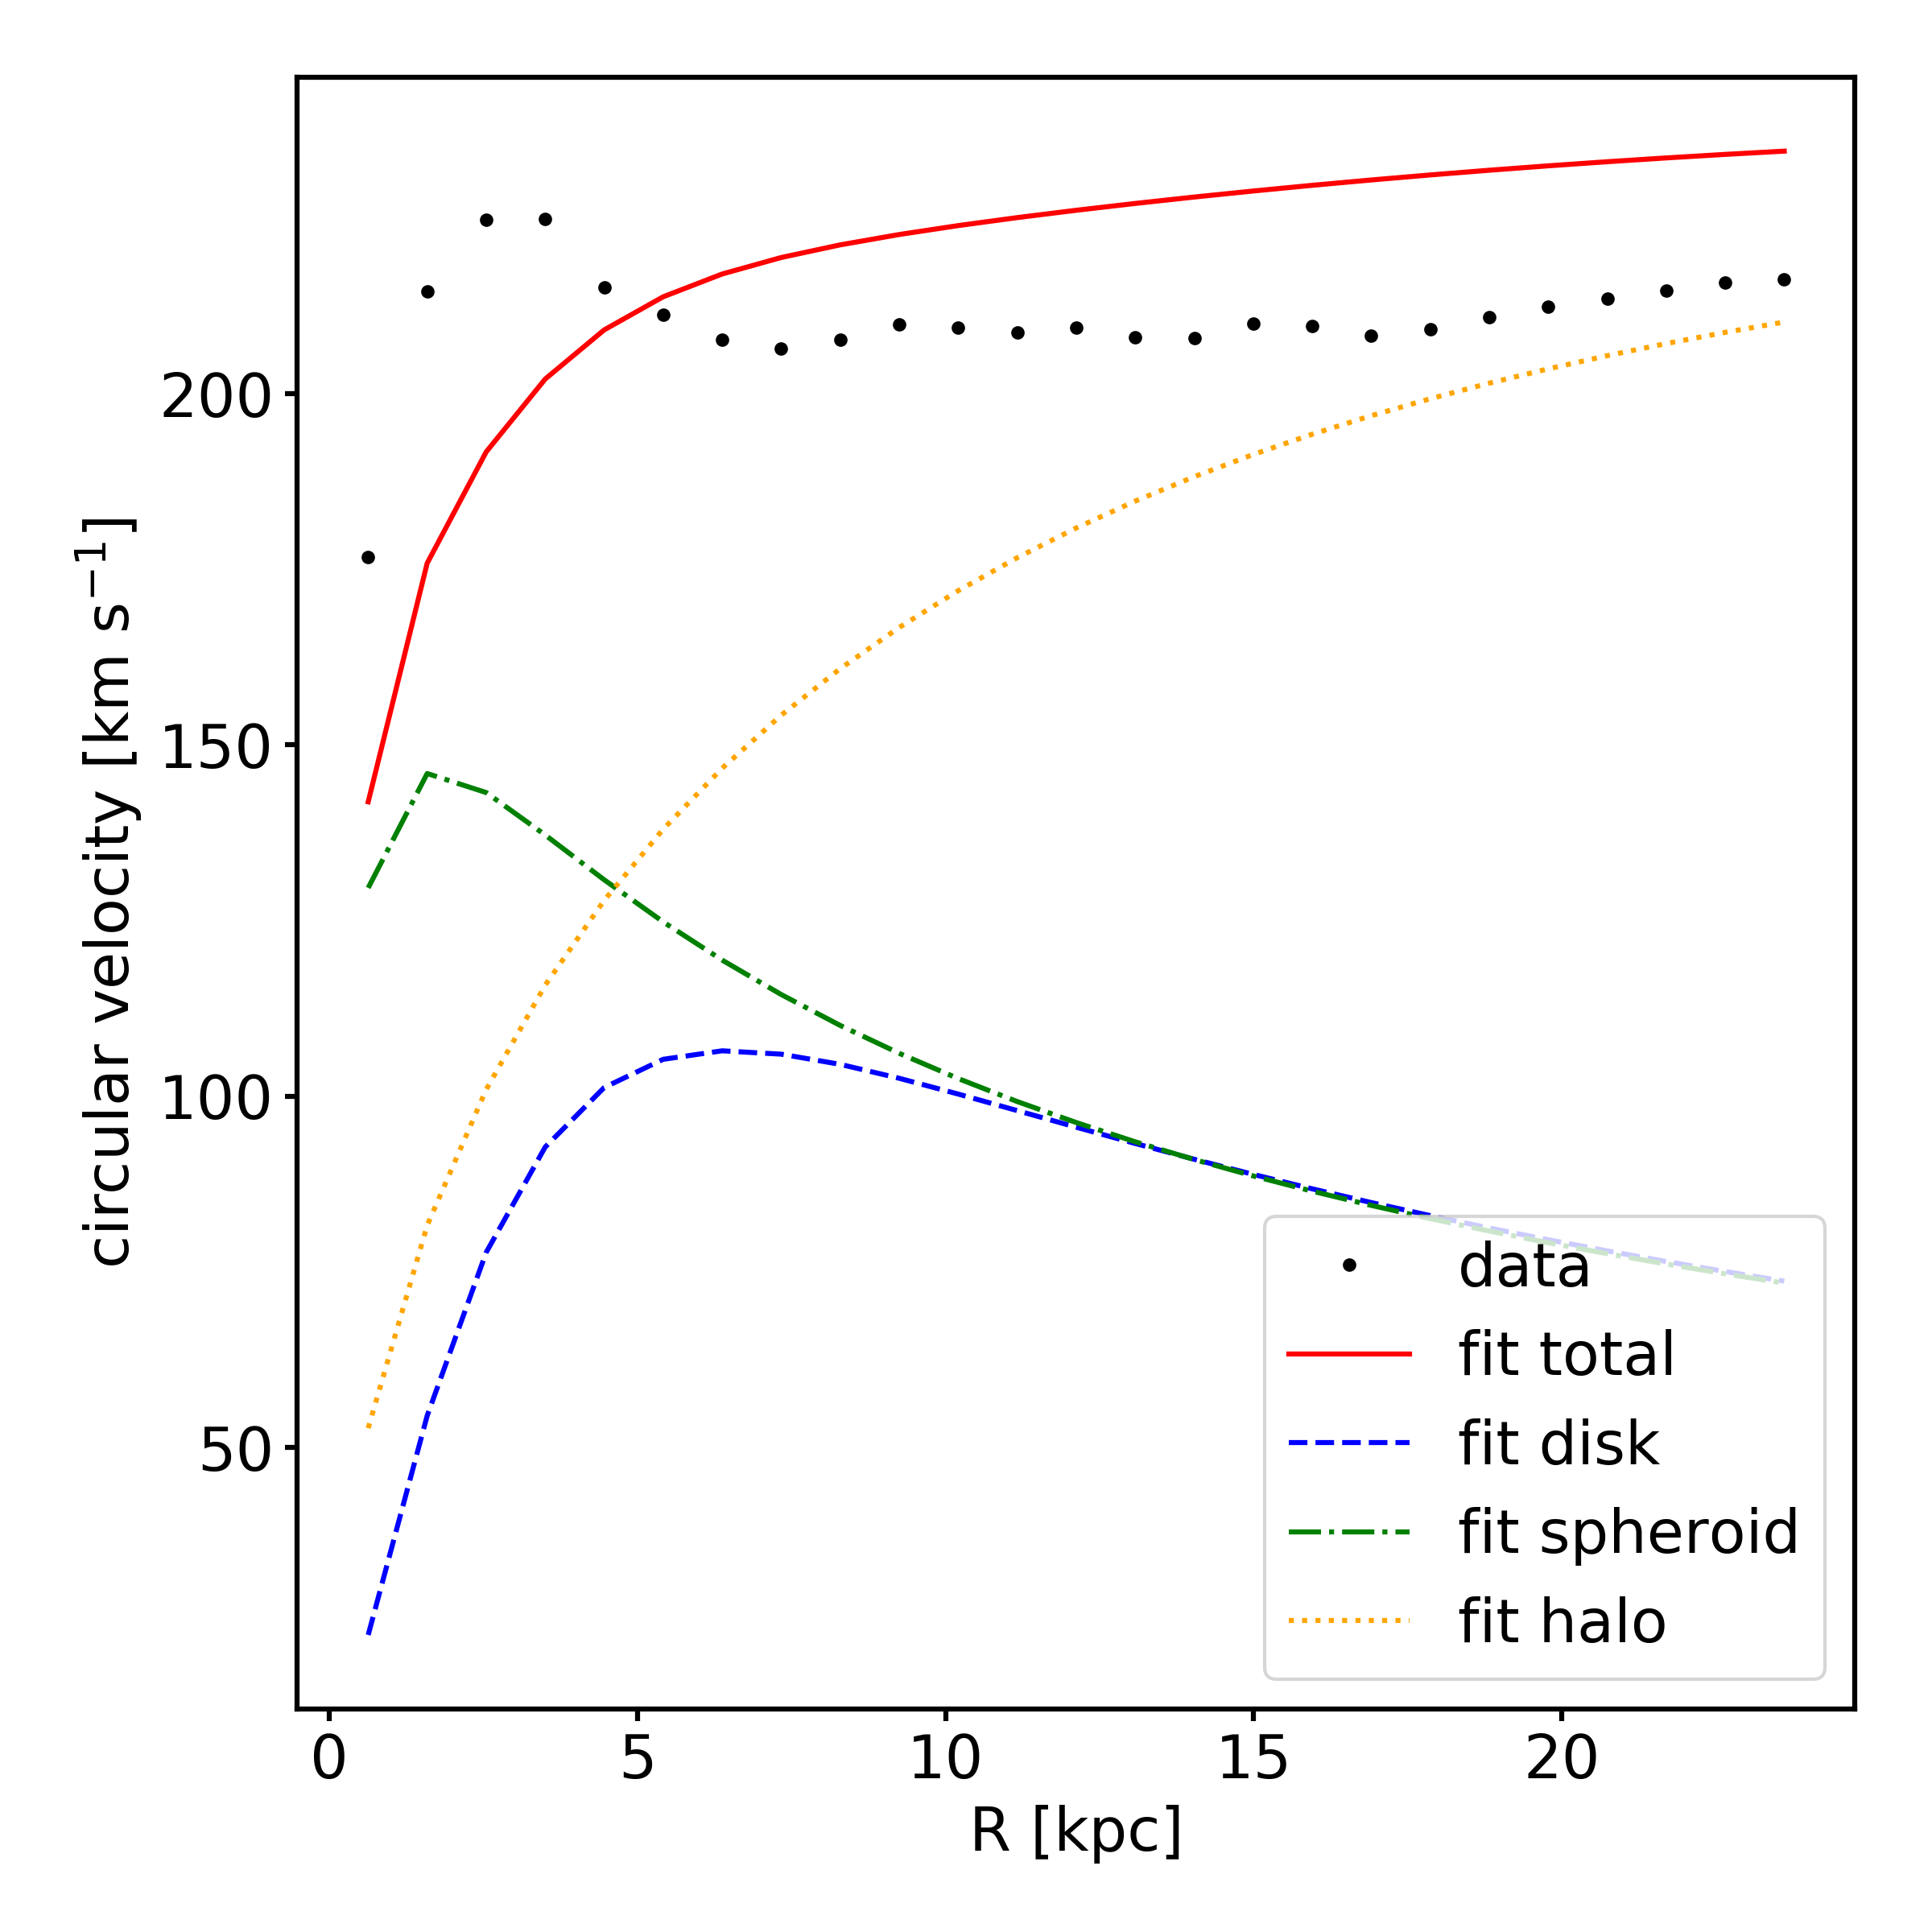
\includegraphics[width=0.5\textwidth]{plots/Auriga/circ_vel_fit_data_test.png}
	\caption{Circular velocity at \textit{z} = 0: data, total, disk, bulge and halo..}
	\label{fig:circ_vel_fit}
\end{figure}

\begin{figure}[htbp]
\centering
	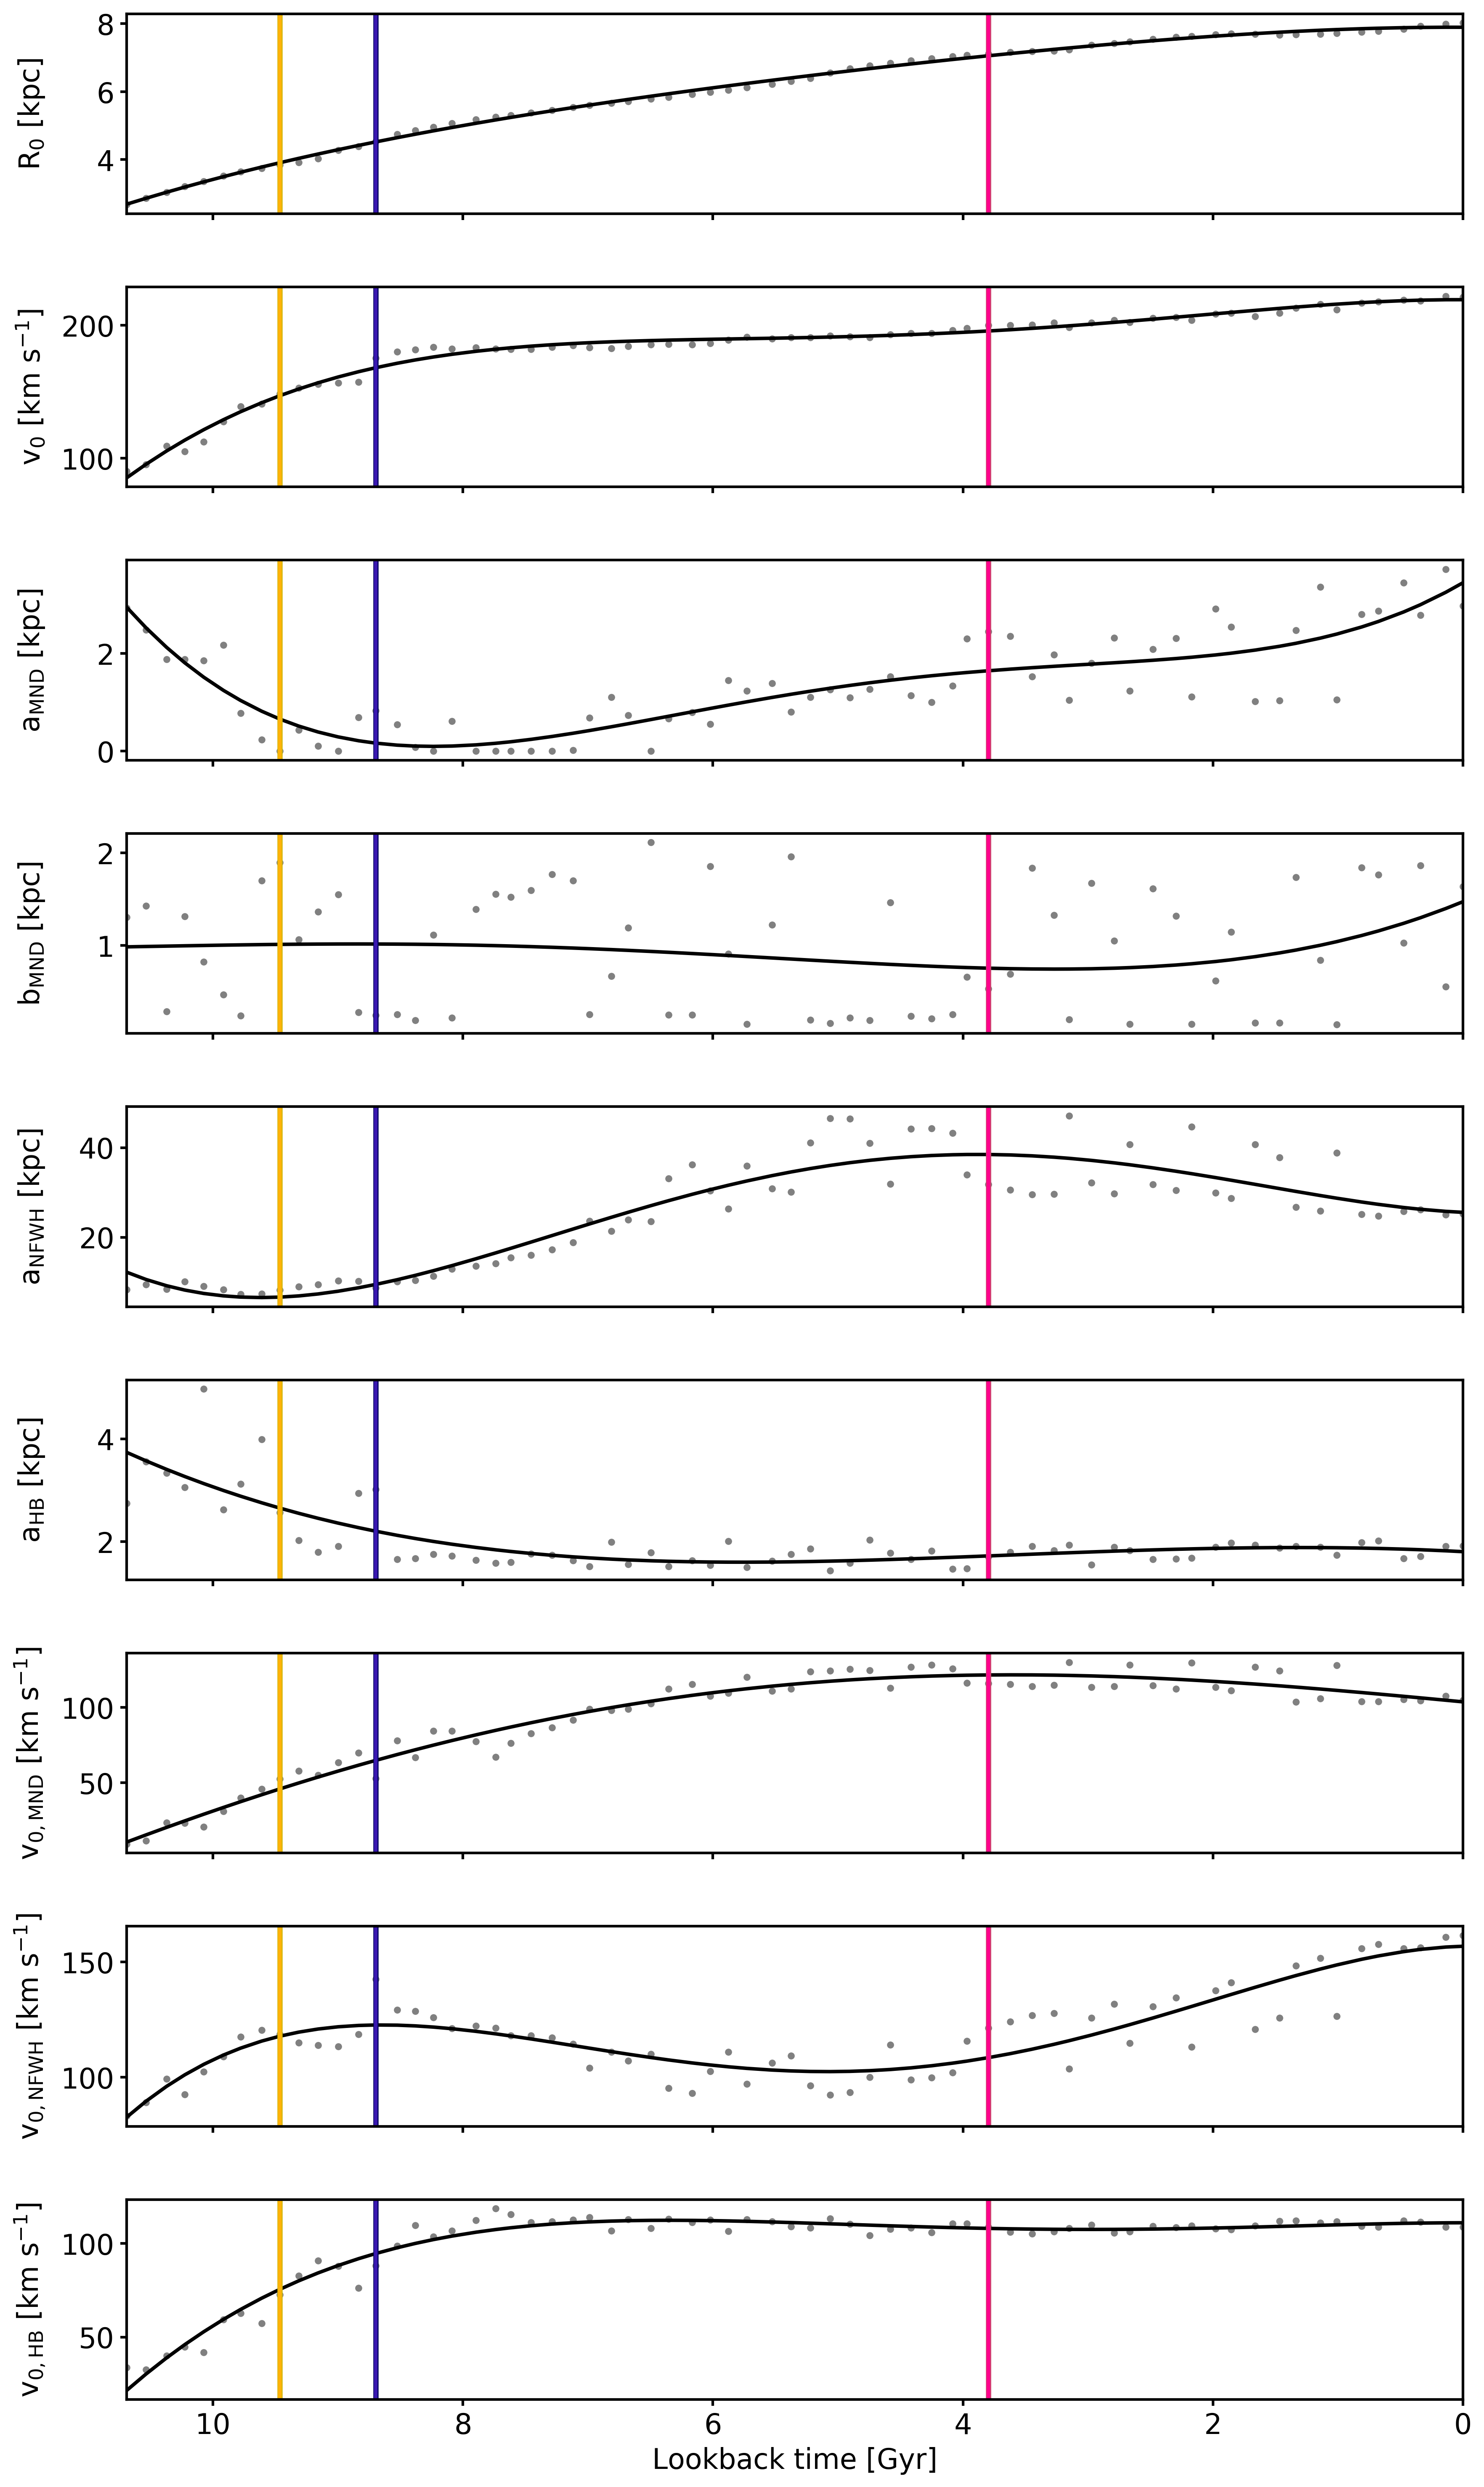
\includegraphics[width=0.9\textwidth]{plots/Auriga/fitted_potential_evolution_dec18.png}
	\caption{Evolution of all fit parameters over time.}
	\label{fig:pot_val_evol}
\end{figure}

\subsection{What not to do when fitting a gravitational potential}



%\subsection{Globular clusters and mass distribution}


